% Options for packages loaded elsewhere
% Options for packages loaded elsewhere
\PassOptionsToPackage{unicode}{hyperref}
\PassOptionsToPackage{hyphens}{url}
\PassOptionsToPackage{dvipsnames,svgnames,x11names}{xcolor}
%
\documentclass[
  letterpaper,
  DIV=11,
  numbers=noendperiod]{scrartcl}
\usepackage{xcolor}
\usepackage{amsmath,amssymb}
\setcounter{secnumdepth}{-\maxdimen} % remove section numbering
\usepackage{iftex}
\ifPDFTeX
  \usepackage[T1]{fontenc}
  \usepackage[utf8]{inputenc}
  \usepackage{textcomp} % provide euro and other symbols
\else % if luatex or xetex
  \usepackage{unicode-math} % this also loads fontspec
  \defaultfontfeatures{Scale=MatchLowercase}
  \defaultfontfeatures[\rmfamily]{Ligatures=TeX,Scale=1}
\fi
\usepackage{lmodern}
\ifPDFTeX\else
  % xetex/luatex font selection
\fi
% Use upquote if available, for straight quotes in verbatim environments
\IfFileExists{upquote.sty}{\usepackage{upquote}}{}
\IfFileExists{microtype.sty}{% use microtype if available
  \usepackage[]{microtype}
  \UseMicrotypeSet[protrusion]{basicmath} % disable protrusion for tt fonts
}{}
\makeatletter
\@ifundefined{KOMAClassName}{% if non-KOMA class
  \IfFileExists{parskip.sty}{%
    \usepackage{parskip}
  }{% else
    \setlength{\parindent}{0pt}
    \setlength{\parskip}{6pt plus 2pt minus 1pt}}
}{% if KOMA class
  \KOMAoptions{parskip=half}}
\makeatother
% Make \paragraph and \subparagraph free-standing
\makeatletter
\ifx\paragraph\undefined\else
  \let\oldparagraph\paragraph
  \renewcommand{\paragraph}{
    \@ifstar
      \xxxParagraphStar
      \xxxParagraphNoStar
  }
  \newcommand{\xxxParagraphStar}[1]{\oldparagraph*{#1}\mbox{}}
  \newcommand{\xxxParagraphNoStar}[1]{\oldparagraph{#1}\mbox{}}
\fi
\ifx\subparagraph\undefined\else
  \let\oldsubparagraph\subparagraph
  \renewcommand{\subparagraph}{
    \@ifstar
      \xxxSubParagraphStar
      \xxxSubParagraphNoStar
  }
  \newcommand{\xxxSubParagraphStar}[1]{\oldsubparagraph*{#1}\mbox{}}
  \newcommand{\xxxSubParagraphNoStar}[1]{\oldsubparagraph{#1}\mbox{}}
\fi
\makeatother

\usepackage{color}
\usepackage{fancyvrb}
\newcommand{\VerbBar}{|}
\newcommand{\VERB}{\Verb[commandchars=\\\{\}]}
\DefineVerbatimEnvironment{Highlighting}{Verbatim}{commandchars=\\\{\}}
% Add ',fontsize=\small' for more characters per line
\usepackage{framed}
\definecolor{shadecolor}{RGB}{241,243,245}
\newenvironment{Shaded}{\begin{snugshade}}{\end{snugshade}}
\newcommand{\AlertTok}[1]{\textcolor[rgb]{0.68,0.00,0.00}{#1}}
\newcommand{\AnnotationTok}[1]{\textcolor[rgb]{0.37,0.37,0.37}{#1}}
\newcommand{\AttributeTok}[1]{\textcolor[rgb]{0.40,0.45,0.13}{#1}}
\newcommand{\BaseNTok}[1]{\textcolor[rgb]{0.68,0.00,0.00}{#1}}
\newcommand{\BuiltInTok}[1]{\textcolor[rgb]{0.00,0.23,0.31}{#1}}
\newcommand{\CharTok}[1]{\textcolor[rgb]{0.13,0.47,0.30}{#1}}
\newcommand{\CommentTok}[1]{\textcolor[rgb]{0.37,0.37,0.37}{#1}}
\newcommand{\CommentVarTok}[1]{\textcolor[rgb]{0.37,0.37,0.37}{\textit{#1}}}
\newcommand{\ConstantTok}[1]{\textcolor[rgb]{0.56,0.35,0.01}{#1}}
\newcommand{\ControlFlowTok}[1]{\textcolor[rgb]{0.00,0.23,0.31}{\textbf{#1}}}
\newcommand{\DataTypeTok}[1]{\textcolor[rgb]{0.68,0.00,0.00}{#1}}
\newcommand{\DecValTok}[1]{\textcolor[rgb]{0.68,0.00,0.00}{#1}}
\newcommand{\DocumentationTok}[1]{\textcolor[rgb]{0.37,0.37,0.37}{\textit{#1}}}
\newcommand{\ErrorTok}[1]{\textcolor[rgb]{0.68,0.00,0.00}{#1}}
\newcommand{\ExtensionTok}[1]{\textcolor[rgb]{0.00,0.23,0.31}{#1}}
\newcommand{\FloatTok}[1]{\textcolor[rgb]{0.68,0.00,0.00}{#1}}
\newcommand{\FunctionTok}[1]{\textcolor[rgb]{0.28,0.35,0.67}{#1}}
\newcommand{\ImportTok}[1]{\textcolor[rgb]{0.00,0.46,0.62}{#1}}
\newcommand{\InformationTok}[1]{\textcolor[rgb]{0.37,0.37,0.37}{#1}}
\newcommand{\KeywordTok}[1]{\textcolor[rgb]{0.00,0.23,0.31}{\textbf{#1}}}
\newcommand{\NormalTok}[1]{\textcolor[rgb]{0.00,0.23,0.31}{#1}}
\newcommand{\OperatorTok}[1]{\textcolor[rgb]{0.37,0.37,0.37}{#1}}
\newcommand{\OtherTok}[1]{\textcolor[rgb]{0.00,0.23,0.31}{#1}}
\newcommand{\PreprocessorTok}[1]{\textcolor[rgb]{0.68,0.00,0.00}{#1}}
\newcommand{\RegionMarkerTok}[1]{\textcolor[rgb]{0.00,0.23,0.31}{#1}}
\newcommand{\SpecialCharTok}[1]{\textcolor[rgb]{0.37,0.37,0.37}{#1}}
\newcommand{\SpecialStringTok}[1]{\textcolor[rgb]{0.13,0.47,0.30}{#1}}
\newcommand{\StringTok}[1]{\textcolor[rgb]{0.13,0.47,0.30}{#1}}
\newcommand{\VariableTok}[1]{\textcolor[rgb]{0.07,0.07,0.07}{#1}}
\newcommand{\VerbatimStringTok}[1]{\textcolor[rgb]{0.13,0.47,0.30}{#1}}
\newcommand{\WarningTok}[1]{\textcolor[rgb]{0.37,0.37,0.37}{\textit{#1}}}

\usepackage{longtable,booktabs,array}
\usepackage{calc} % for calculating minipage widths
% Correct order of tables after \paragraph or \subparagraph
\usepackage{etoolbox}
\makeatletter
\patchcmd\longtable{\par}{\if@noskipsec\mbox{}\fi\par}{}{}
\makeatother
% Allow footnotes in longtable head/foot
\IfFileExists{footnotehyper.sty}{\usepackage{footnotehyper}}{\usepackage{footnote}}
\makesavenoteenv{longtable}
\usepackage{graphicx}
\makeatletter
\newsavebox\pandoc@box
\newcommand*\pandocbounded[1]{% scales image to fit in text height/width
  \sbox\pandoc@box{#1}%
  \Gscale@div\@tempa{\textheight}{\dimexpr\ht\pandoc@box+\dp\pandoc@box\relax}%
  \Gscale@div\@tempb{\linewidth}{\wd\pandoc@box}%
  \ifdim\@tempb\p@<\@tempa\p@\let\@tempa\@tempb\fi% select the smaller of both
  \ifdim\@tempa\p@<\p@\scalebox{\@tempa}{\usebox\pandoc@box}%
  \else\usebox{\pandoc@box}%
  \fi%
}
% Set default figure placement to htbp
\def\fps@figure{htbp}
\makeatother





\setlength{\emergencystretch}{3em} % prevent overfull lines

\providecommand{\tightlist}{%
  \setlength{\itemsep}{0pt}\setlength{\parskip}{0pt}}



 


\KOMAoption{captions}{tableheading}
\makeatletter
\@ifpackageloaded{caption}{}{\usepackage{caption}}
\AtBeginDocument{%
\ifdefined\contentsname
  \renewcommand*\contentsname{Table of contents}
\else
  \newcommand\contentsname{Table of contents}
\fi
\ifdefined\listfigurename
  \renewcommand*\listfigurename{List of Figures}
\else
  \newcommand\listfigurename{List of Figures}
\fi
\ifdefined\listtablename
  \renewcommand*\listtablename{List of Tables}
\else
  \newcommand\listtablename{List of Tables}
\fi
\ifdefined\figurename
  \renewcommand*\figurename{Figure}
\else
  \newcommand\figurename{Figure}
\fi
\ifdefined\tablename
  \renewcommand*\tablename{Table}
\else
  \newcommand\tablename{Table}
\fi
}
\@ifpackageloaded{float}{}{\usepackage{float}}
\floatstyle{ruled}
\@ifundefined{c@chapter}{\newfloat{codelisting}{h}{lop}}{\newfloat{codelisting}{h}{lop}[chapter]}
\floatname{codelisting}{Listing}
\newcommand*\listoflistings{\listof{codelisting}{List of Listings}}
\makeatother
\makeatletter
\makeatother
\makeatletter
\@ifpackageloaded{caption}{}{\usepackage{caption}}
\@ifpackageloaded{subcaption}{}{\usepackage{subcaption}}
\makeatother
\usepackage{bookmark}
\IfFileExists{xurl.sty}{\usepackage{xurl}}{} % add URL line breaks if available
\urlstyle{same}
\hypersetup{
  pdftitle={Importing libraries},
  colorlinks=true,
  linkcolor={blue},
  filecolor={Maroon},
  citecolor={Blue},
  urlcolor={Blue},
  pdfcreator={LaTeX via pandoc}}


\title{Importing libraries}
\author{}
\date{}
\begin{document}
\maketitle


\section{Python Libraries
Description}\label{python-libraries-description}

\subsection{Overview}\label{overview}

This markdown describes Python libraries commonly used in Jupyter
Notebooks for data analysis, visualization, and machine learning.

\subsection{Library Descriptions}\label{library-descriptions}

\begin{itemize}
\tightlist
\item
  \textbf{numpy}: Handles numerical computations with arrays and
  matrices.
\item
  \textbf{pandas}: Manages and analyzes data using DataFrames.
\item
  \textbf{matplotlib.pyplot}: Generates plots and visualizations.
\item
  \textbf{seaborn}: Creates enhanced statistical visualizations.
\item
  \textbf{tensorflow}: Supports building and training machine learning
  models.
\item
  \textbf{tensorflow}: A comprehensive platform for building and
  training machine learning models.

  \begin{itemize}
  \tightlist
  \item
    \textbf{tensorflow.keras}: A high-level API within TensorFlow for
    building and training deep learning models (e.g.,
    \texttt{Sequential}, \texttt{Dense}, \texttt{Dropout}).
  \end{itemize}
\item
  \textbf{scikit-learn (sklearn)}: A powerful and widely used library
  for classical machine learning. It includes modules for:

  \begin{itemize}
  \tightlist
  \item
    \textbf{Preprocessing}: (e.g., \texttt{LabelEncoder},
    \texttt{StandardScaler})
  \item
    \textbf{Model Selection}: (e.g., \texttt{train\_test\_split})
  \item
    \textbf{Models}: (e.g., \texttt{LogisticRegression})
  \item
    \textbf{Metrics}: (e.g., \texttt{accuracy\_score},
    \texttt{classification\_report})
  \end{itemize}
\item
  \textbf{lime}: Stands for Local Interpretable Model-agnostic
  Explanations. It's a library used to explain the predictions of any
  machine learning model.
\item
  \textbf{shap}: (SHapley Additive exPlanations) A library for
  explaining the output of machine learning models, providing insights
  into feature importance and prediction logic.
\end{itemize}

\subsection{Purpose}\label{purpose}

These libraries enable efficient data processing, visualization, and
machine learning model development in Jupyter Notebooks, using standard
aliases for concise coding.

\begin{Shaded}
\begin{Highlighting}[]
\ImportTok{import}\NormalTok{ shap}
\ImportTok{import}\NormalTok{ numpy }\ImportTok{as}\NormalTok{ np}
\ImportTok{import}\NormalTok{ pandas }\ImportTok{as}\NormalTok{ pd}
\ImportTok{import}\NormalTok{ matplotlib.pyplot }\ImportTok{as}\NormalTok{ plt}
\ImportTok{import}\NormalTok{ seaborn }\ImportTok{as}\NormalTok{ sns}
\ImportTok{import}\NormalTok{ tensorflow }\ImportTok{as}\NormalTok{ tf}
\ImportTok{from}\NormalTok{ sklearn.model\_selection }\ImportTok{import}\NormalTok{ train\_test\_split}
\ImportTok{from}\NormalTok{ sklearn.linear\_model }\ImportTok{import}\NormalTok{ LogisticRegression}
\ImportTok{from}\NormalTok{ tensorflow.keras.models }\ImportTok{import}\NormalTok{ Sequential}
\ImportTok{from}\NormalTok{ tensorflow.keras.layers }\ImportTok{import}\NormalTok{ Dense, Dropout}
\ImportTok{from}\NormalTok{ tensorflow.keras.utils }\ImportTok{import}\NormalTok{ to\_categorical}
\ImportTok{from}\NormalTok{ sklearn.preprocessing }\ImportTok{import}\NormalTok{ LabelEncoder, StandardScaler}
\ImportTok{from}\NormalTok{ lime }\ImportTok{import}\NormalTok{ lime\_tabular}
\ImportTok{from}\NormalTok{ lime.lime\_tabular }\ImportTok{import}\NormalTok{ LimeTabularExplainer}
\ImportTok{from}\NormalTok{ sklearn.metrics }\ImportTok{import}\NormalTok{ accuracy\_score, precision\_score, recall\_score, f1\_score, classification\_report}
\end{Highlighting}
\end{Shaded}

\section{Loading and Preparing Data in Jupyter
Notebook}\label{loading-and-preparing-data-in-jupyter-notebook}

\subsection{Overview}\label{overview-1}

This Python code loads three CSV files into pandas DataFrames and then
renames specific columns to prevent naming conflicts, preparing the data
for analysis in a Jupyter Notebook.

\subsection{Code Description}\label{code-description}

\begin{itemize}
\tightlist
\item
  \textbf{\texttt{hotels\ =\ pd.read\_csv(...)}}: Loads hotel data from
  a CSV file into a DataFrame named \texttt{hotels}.
\item
  \textbf{\texttt{reviews\ =\ pd.read\_csv(...)}}: Loads review data
  from a CSV file into a DataFrame named \texttt{reviews}.
\item
  \textbf{\texttt{users\ =\ pd.read\_csv(...)}}: Loads user data from a
  CSV file into a DataFrame named \texttt{users}.
\item
  \textbf{\texttt{hotels\ =\ hotels.rename(...)}}: Renames the
  \texttt{country} column in the \texttt{hotels} DataFrame to
  \texttt{hotel\_country}.
\item
  \textbf{\texttt{users\ =\ users.rename(...)}}: Renames the
  \texttt{country} column in the \texttt{users} DataFrame to
  \texttt{user\_country}.
\end{itemize}

\subsection{Purpose}\label{purpose-1}

This code imports datasets into pandas DataFrames. It also performs
initial data cleaning by \textbf{renaming the `country' columns} in the
\texttt{hotels} and \texttt{users} tables. This is a crucial step to
avoid ambiguity and prevent column name collisions before merging these
DataFrames.

\begin{Shaded}
\begin{Highlighting}[]
\NormalTok{hotels}\OperatorTok{=}\NormalTok{pd.read\_csv(}\StringTok{"C:/Users/abdel/ACL/archive/hotels.csv"}\NormalTok{)}
\NormalTok{reviews}\OperatorTok{=}\NormalTok{pd.read\_csv(}\StringTok{"C:/Users/abdel/ACL/archive/reviews.csv"}\NormalTok{)}
\NormalTok{users}\OperatorTok{=}\NormalTok{pd.read\_csv(}\StringTok{"C:/Users/abdel/ACL/archive/users.csv"}\NormalTok{)}
\NormalTok{hotels }\OperatorTok{=}\NormalTok{ hotels.rename(columns}\OperatorTok{=}\NormalTok{\{}\StringTok{\textquotesingle{}country\textquotesingle{}}\NormalTok{: }\StringTok{\textquotesingle{}hotel\_country\textquotesingle{}}\NormalTok{\})}
\NormalTok{users }\OperatorTok{=}\NormalTok{ users.rename(columns}\OperatorTok{=}\NormalTok{\{}\StringTok{\textquotesingle{}country\textquotesingle{}}\NormalTok{: }\StringTok{\textquotesingle{}user\_country\textquotesingle{}}\NormalTok{\})}
\end{Highlighting}
\end{Shaded}

\subsubsection{🔍 Data Quality Check}\label{data-quality-check}

This cell checks for duplicates and missing values in the
\textbf{Hotels}, \textbf{Reviews}, and \textbf{Users} datasets using
\texttt{duplicated()} and \texttt{isnull().sum()}.\\
It was found that there are \textbf{no duplicate records} and \textbf{no
missing values} in any of the datasets.

\begin{Shaded}
\begin{Highlighting}[]
\BuiltInTok{print}\NormalTok{(}\SpecialStringTok{f"Hotels duplicates: }\SpecialCharTok{\{}\NormalTok{hotels}\SpecialCharTok{.}\NormalTok{duplicated()}\SpecialCharTok{.}\BuiltInTok{sum}\NormalTok{()}\SpecialCharTok{\}}\SpecialStringTok{"}\NormalTok{)}
\BuiltInTok{print}\NormalTok{(}\SpecialStringTok{f"Reviews duplicates: }\SpecialCharTok{\{}\NormalTok{reviews}\SpecialCharTok{.}\NormalTok{duplicated()}\SpecialCharTok{.}\BuiltInTok{sum}\NormalTok{()}\SpecialCharTok{\}}\SpecialStringTok{"}\NormalTok{)}
\BuiltInTok{print}\NormalTok{(}\SpecialStringTok{f"Users duplicates: }\SpecialCharTok{\{}\NormalTok{users}\SpecialCharTok{.}\NormalTok{duplicated()}\SpecialCharTok{.}\BuiltInTok{sum}\NormalTok{()}\SpecialCharTok{\}}\SpecialStringTok{"}\NormalTok{)}
\BuiltInTok{print}\NormalTok{(}\StringTok{"{-}{-}{-}{-}{-}{-}{-}{-}{-}{-}{-}{-}{-}{-}{-}{-}{-}{-}{-}{-}{-}{-}{-}{-}{-}{-}{-}{-}{-}{-}{-}{-}"}\NormalTok{)}
\BuiltInTok{print}\NormalTok{(}\SpecialStringTok{f"Hotels nuls: }\SpecialCharTok{\{}\NormalTok{hotels}\SpecialCharTok{.}\NormalTok{isnull()}\SpecialCharTok{.}\BuiltInTok{sum}\NormalTok{()}\SpecialCharTok{\}}\SpecialStringTok{"}\NormalTok{)}
\BuiltInTok{print}\NormalTok{(}\StringTok{"{-}{-}{-}{-}{-}{-}{-}{-}{-}{-}{-}{-}{-}{-}{-}{-}{-}{-}{-}{-}{-}{-}{-}{-}{-}{-}{-}{-}{-}{-}{-}{-}"}\NormalTok{)}
\BuiltInTok{print}\NormalTok{(}\SpecialStringTok{f"Reviews nuls: }\SpecialCharTok{\{}\NormalTok{reviews}\SpecialCharTok{.}\NormalTok{isnull()}\SpecialCharTok{.}\BuiltInTok{sum}\NormalTok{()}\SpecialCharTok{\}}\SpecialStringTok{"}\NormalTok{)}
\BuiltInTok{print}\NormalTok{(}\StringTok{"{-}{-}{-}{-}{-}{-}{-}{-}{-}{-}{-}{-}{-}{-}{-}{-}{-}{-}{-}{-}{-}{-}{-}{-}{-}{-}{-}{-}{-}{-}{-}{-}"}\NormalTok{)}
\BuiltInTok{print}\NormalTok{(}\SpecialStringTok{f"Users nuls: }\SpecialCharTok{\{}\NormalTok{users}\SpecialCharTok{.}\NormalTok{isnull()}\SpecialCharTok{.}\BuiltInTok{sum}\NormalTok{()}\SpecialCharTok{\}}\SpecialStringTok{"}\NormalTok{)}
\end{Highlighting}
\end{Shaded}

\begin{verbatim}
Hotels duplicates: 0
Reviews duplicates: 0
Users duplicates: 0
--------------------------------
Hotels nuls: hotel_id                0
hotel_name              0
city                    0
hotel_country           0
star_rating             0
lat                     0
lon                     0
cleanliness_base        0
comfort_base            0
facilities_base         0
location_base           0
staff_base              0
value_for_money_base    0
dtype: int64
--------------------------------
Reviews nuls: review_id                0
user_id                  0
hotel_id                 0
review_date              0
score_overall            0
score_cleanliness        0
score_comfort            0
score_facilities         0
score_location           0
score_staff              0
score_value_for_money    0
review_text              0
dtype: int64
--------------------------------
Users nuls: user_id           0
user_gender       0
user_country      0
age_group         0
traveller_type    0
join_date         0
dtype: int64
\end{verbatim}

\subsubsection{🧾 Dataset Overview}\label{dataset-overview}

This cell displays the structure and summary information of the
\textbf{Reviews}, \textbf{Hotels}, and \textbf{Users} datasets using
\texttt{info()}.\\
It shows the number of entries, column names, data types, and confirms
that there are \textbf{no missing values} in any dataset.

\begin{Shaded}
\begin{Highlighting}[]
\NormalTok{reviews.info()}
\BuiltInTok{print}\NormalTok{(}\StringTok{"{-}{-}{-}{-}{-}{-}{-}{-}{-}{-}{-}{-}{-}{-}{-}{-}{-}{-}{-}{-}{-}{-}{-}{-}{-}{-}{-}{-}{-}{-}{-}{-}"}\NormalTok{)   }
\NormalTok{hotels.info()}
\BuiltInTok{print}\NormalTok{(}\StringTok{"{-}{-}{-}{-}{-}{-}{-}{-}{-}{-}{-}{-}{-}{-}{-}{-}{-}{-}{-}{-}{-}{-}{-}{-}{-}{-}{-}{-}{-}{-}{-}{-}"}\NormalTok{)}
\NormalTok{users.info()}
\BuiltInTok{print}\NormalTok{(}\StringTok{"{-}{-}{-}{-}{-}{-}{-}{-}{-}{-}{-}{-}{-}{-}{-}{-}{-}{-}{-}{-}{-}{-}{-}{-}{-}{-}{-}{-}{-}{-}{-}{-}"}\NormalTok{)}
\end{Highlighting}
\end{Shaded}

\begin{verbatim}
<class 'pandas.core.frame.DataFrame'>
RangeIndex: 50000 entries, 0 to 49999
Data columns (total 12 columns):
 #   Column                 Non-Null Count  Dtype  
---  ------                 --------------  -----  
 0   review_id              50000 non-null  int64  
 1   user_id                50000 non-null  int64  
 2   hotel_id               50000 non-null  int64  
 3   review_date            50000 non-null  object 
 4   score_overall          50000 non-null  float64
 5   score_cleanliness      50000 non-null  float64
 6   score_comfort          50000 non-null  float64
 7   score_facilities       50000 non-null  float64
 8   score_location         50000 non-null  float64
 9   score_staff            50000 non-null  float64
 10  score_value_for_money  50000 non-null  float64
 11  review_text            50000 non-null  object 
dtypes: float64(7), int64(3), object(2)
memory usage: 4.6+ MB
--------------------------------
<class 'pandas.core.frame.DataFrame'>
RangeIndex: 25 entries, 0 to 24
Data columns (total 13 columns):
 #   Column                Non-Null Count  Dtype  
---  ------                --------------  -----  
 0   hotel_id              25 non-null     int64  
 1   hotel_name            25 non-null     object 
 2   city                  25 non-null     object 
 3   hotel_country         25 non-null     object 
 4   star_rating           25 non-null     int64  
 5   lat                   25 non-null     float64
 6   lon                   25 non-null     float64
 7   cleanliness_base      25 non-null     float64
 8   comfort_base          25 non-null     float64
 9   facilities_base       25 non-null     float64
 10  location_base         25 non-null     float64
 11  staff_base            25 non-null     float64
 12  value_for_money_base  25 non-null     float64
dtypes: float64(8), int64(2), object(3)
memory usage: 2.7+ KB
--------------------------------
<class 'pandas.core.frame.DataFrame'>
RangeIndex: 2000 entries, 0 to 1999
Data columns (total 6 columns):
 #   Column          Non-Null Count  Dtype 
---  ------          --------------  ----- 
 0   user_id         2000 non-null   int64 
 1   user_gender     2000 non-null   object
 2   user_country    2000 non-null   object
 3   age_group       2000 non-null   object
 4   traveller_type  2000 non-null   object
 5   join_date       2000 non-null   object
dtypes: int64(1), object(5)
memory usage: 93.9+ KB
--------------------------------
\end{verbatim}

\section{Merging DataFrames}\label{merging-dataframes}

\subsection{Overview}\label{overview-2}

Merges pandas DataFrames (\texttt{reviews}, \texttt{hotels},
\texttt{users}) for analysis in Jupyter Notebook.

\subsection{Description}\label{description}

\begin{itemize}
\tightlist
\item
  \textbf{\texttt{review\_hotel\_df\ =\ reviews.merge(hotels,\ on=\textquotesingle{}hotel\_id\textquotesingle{},\ how=\textquotesingle{}left\textquotesingle{})}}:
  Merges \texttt{reviews} with \texttt{hotels} on \texttt{hotel\_id}
  using left join.
\item
  \textbf{\texttt{df\ =\ review\_hotel\_df.merge(users,\ on=\textquotesingle{}user\_id\textquotesingle{},\ how=\textquotesingle{}left\textquotesingle{})}}:
  Merges \texttt{review\_hotel\_df} with \texttt{users} on
  \texttt{user\_id} using left join.
\end{itemize}

\subsection{Purpose}\label{purpose-2}

Combines review, hotel, and user data into one DataFrame for integrated
analysis.

\begin{Shaded}
\begin{Highlighting}[]
\NormalTok{review\_hotel\_df}\OperatorTok{=}\NormalTok{reviews.merge(hotels,on}\OperatorTok{=}\StringTok{\textquotesingle{}hotel\_id\textquotesingle{}}\NormalTok{,how}\OperatorTok{=}\StringTok{\textquotesingle{}left\textquotesingle{}}\NormalTok{)}
\NormalTok{df}\OperatorTok{=}\NormalTok{review\_hotel\_df.merge(users,on}\OperatorTok{=}\StringTok{\textquotesingle{}user\_id\textquotesingle{}}\NormalTok{,how}\OperatorTok{=}\StringTok{\textquotesingle{}left\textquotesingle{}}\NormalTok{)}
\end{Highlighting}
\end{Shaded}

\subsection{Data Integrity Check: Verifying Row Count and Nulls in Key
Columns (Features about the
user)}\label{data-integrity-check-verifying-row-count-and-nulls-in-key-columns-features-about-the-user}

\begin{Shaded}
\begin{Highlighting}[]
\BuiltInTok{print}\NormalTok{(}\SpecialStringTok{f"Total rows in df (should be \textasciitilde{}50,000): }\SpecialCharTok{\{}\BuiltInTok{len}\NormalTok{(df)}\SpecialCharTok{\}}\SpecialStringTok{"}\NormalTok{)}
\BuiltInTok{print}\NormalTok{(}\StringTok{"}\CharTok{\textbackslash{}n}\StringTok{Null values *after* merge:"}\NormalTok{)}
\BuiltInTok{print}\NormalTok{(df[[}\StringTok{\textquotesingle{}user\_gender\textquotesingle{}}\NormalTok{, }\StringTok{\textquotesingle{}age\_group\textquotesingle{}}\NormalTok{, }\StringTok{\textquotesingle{}traveller\_type\textquotesingle{}}\NormalTok{]].isnull().}\BuiltInTok{sum}\NormalTok{())}
\end{Highlighting}
\end{Shaded}

\begin{verbatim}
Total rows in df (should be ~50,000): 50000

Null values *after* merge:
user_gender       0
age_group         0
traveller_type    0
dtype: int64
\end{verbatim}

\section{Country Grouping in
DataFrame}\label{country-grouping-in-dataframe}

\subsection{Overview}\label{overview-3}

Assigns country groups to hotels based on their country and displays
selected columns.

\subsection{Description}\label{description-1}

\begin{itemize}
\tightlist
\item
  \textbf{\texttt{groups\ =\ \{...\}}}: Defines a dictionary mapping
  regions to lists of countries (e.g., North\_America: United States,
  Canada).
\item
  \textbf{\texttt{df{[}"country\_group"{]}\ =\ df{[}"hotel\_country"{]}.apply(...)}}:
  Creates a \texttt{country\_group} column by mapping
  \texttt{hotel\_country} to a region from \texttt{groups}, defaulting
  to ``Other'' if not found.
\item
  \textbf{\texttt{df{[}{[}"hotel\_country","user\_country","country\_group"{]}{]}}}:
  Selects \texttt{hotel\_country}, \texttt{user\_country}, and
  \texttt{country\_group} columns for display.
\end{itemize}

\subsection{Purpose}\label{purpose-3}

Categorizes hotels by geographic region and shows relevant country data
to fill country\_group column.

\begin{Shaded}
\begin{Highlighting}[]
\NormalTok{groups}\OperatorTok{=}\NormalTok{\{}\StringTok{\textquotesingle{}North\_America\textquotesingle{}}\NormalTok{:[}\StringTok{\textquotesingle{}United States\textquotesingle{}}\NormalTok{,}\StringTok{\textquotesingle{}Canada\textquotesingle{}}\NormalTok{],}
        \StringTok{\textquotesingle{}Western\_Europe\textquotesingle{}}\NormalTok{:[}\StringTok{\textquotesingle{}Germany\textquotesingle{}}\NormalTok{,}\StringTok{\textquotesingle{}France\textquotesingle{}}\NormalTok{,}\StringTok{\textquotesingle{}United Kingdom\textquotesingle{}}\NormalTok{,}\StringTok{\textquotesingle{}Netherlands\textquotesingle{}}\NormalTok{,}\StringTok{\textquotesingle{}Spain\textquotesingle{}}\NormalTok{,}\StringTok{\textquotesingle{}Italy\textquotesingle{}}\NormalTok{],}
        \StringTok{\textquotesingle{}Eastern\_Europe\textquotesingle{}}\NormalTok{:[}\StringTok{\textquotesingle{}Russia\textquotesingle{}}\NormalTok{],}
        \StringTok{\textquotesingle{}East\_Asia\textquotesingle{}}\NormalTok{:[}\StringTok{\textquotesingle{}China\textquotesingle{}}\NormalTok{,}\StringTok{\textquotesingle{}Japan\textquotesingle{}}\NormalTok{,}\StringTok{\textquotesingle{}South Korea\textquotesingle{}}\NormalTok{],}
        \StringTok{\textquotesingle{}Southeast\_Asia\textquotesingle{}}\NormalTok{:[}\StringTok{\textquotesingle{}Thailand\textquotesingle{}}\NormalTok{,}\StringTok{\textquotesingle{}Singapore\textquotesingle{}}\NormalTok{],}
        \StringTok{\textquotesingle{}Middle\_East\textquotesingle{}}\NormalTok{:[}\StringTok{\textquotesingle{}United Arab Emirates\textquotesingle{}}\NormalTok{,}\StringTok{\textquotesingle{}Turkey\textquotesingle{}}\NormalTok{],}
        \StringTok{\textquotesingle{}Africa\textquotesingle{}}\NormalTok{:[}\StringTok{\textquotesingle{}Egypt\textquotesingle{}}\NormalTok{,}\StringTok{\textquotesingle{}Nigeria\textquotesingle{}}\NormalTok{,}\StringTok{\textquotesingle{}South Africa\textquotesingle{}}\NormalTok{],}
        \StringTok{\textquotesingle{}Oceania\textquotesingle{}}\NormalTok{:[}\StringTok{\textquotesingle{}Australia\textquotesingle{}}\NormalTok{,}\StringTok{\textquotesingle{}New Zealand\textquotesingle{}}\NormalTok{],}
        \StringTok{\textquotesingle{}South\_America\textquotesingle{}}\NormalTok{:[}\StringTok{\textquotesingle{}Brazil\textquotesingle{}}\NormalTok{,}\StringTok{\textquotesingle{}Argentina\textquotesingle{}}\NormalTok{],}
        \StringTok{\textquotesingle{}South\_Asia\textquotesingle{}}\NormalTok{:[}\StringTok{\textquotesingle{}India\textquotesingle{}}\NormalTok{],}
        \StringTok{\textquotesingle{}North\_America\_Mexico\textquotesingle{}}\NormalTok{:[}\StringTok{\textquotesingle{}Mexico\textquotesingle{}}\NormalTok{]\}}

\NormalTok{df[}\StringTok{"country\_group"}\NormalTok{]}\OperatorTok{=}\NormalTok{df[}\StringTok{"hotel\_country"}\NormalTok{].}\BuiltInTok{apply}\NormalTok{(}\KeywordTok{lambda}\NormalTok{ x: }\BuiltInTok{next}\NormalTok{((key }\ControlFlowTok{for}\NormalTok{ key, value }\KeywordTok{in}\NormalTok{ groups.items() }\ControlFlowTok{if}\NormalTok{ x }\KeywordTok{in}\NormalTok{ value), }\StringTok{"Other"}\NormalTok{))}

\NormalTok{df[[}\StringTok{"hotel\_country"}\NormalTok{,}\StringTok{"user\_country"}\NormalTok{,}\StringTok{"country\_group"}\NormalTok{]]}
\end{Highlighting}
\end{Shaded}

\begin{longtable}[]{@{}llll@{}}
\toprule\noalign{}
& hotel\_country & user\_country & country\_group \\
\midrule\noalign{}
\endhead
\bottomrule\noalign{}
\endlastfoot
0 & United States & New Zealand & North\_America \\
1 & Japan & United Kingdom & East\_Asia \\
2 & Egypt & Spain & Africa \\
3 & Spain & United Kingdom & Western\_Europe \\
4 & Russia & Australia & Eastern\_Europe \\
... & ... & ... & ... \\
49995 & Nigeria & Mexico & Africa \\
49996 & Brazil & New Zealand & South\_America \\
49997 & Singapore & Russia & Southeast\_Asia \\
49998 & Turkey & United Kingdom & Middle\_East \\
49999 & Spain & Turkey & Western\_Europe \\
\end{longtable}

\section{Data-Engineering Question 1}\label{data-engineering-question-1}

\subsection{Overview}\label{overview-4}

Calculates the best city for each traveller type based on reviews.

\subsection{Description}\label{description-2}

\begin{itemize}
\tightlist
\item
  \textbf{\texttt{city\_scores\ =\ df.groupby({[}\textquotesingle{}traveller\_type\textquotesingle{},\ \textquotesingle{}city\textquotesingle{}{]}){[}\textquotesingle{}score\_overall\textquotesingle{}{]}.mean().reset\_index().sort\_values(...)}}:
  Groups data by \texttt{traveller\_type} and \texttt{city}, computes
  mean \texttt{score\_overall}, resets index, and sorts by
  \texttt{traveller\_type} (ascending) and \texttt{score\_overall}
  (descending).
\item
  \textbf{\texttt{best\_cities\ =\ city\_scores.groupby(\textquotesingle{}traveller\_type\textquotesingle{}).head(1)}}:
  Selects the top city (highest score) for each
  \texttt{traveller\_type}.
\end{itemize}

\begin{Shaded}
\begin{Highlighting}[]
\NormalTok{city\_scores }\OperatorTok{=}\NormalTok{ df.groupby([}\StringTok{\textquotesingle{}traveller\_type\textquotesingle{}}\NormalTok{, }\StringTok{\textquotesingle{}city\textquotesingle{}}\NormalTok{])[}\StringTok{\textquotesingle{}score\_overall\textquotesingle{}}\NormalTok{].mean().reset\_index().sort\_values([}\StringTok{\textquotesingle{}traveller\_type\textquotesingle{}}\NormalTok{, }\StringTok{\textquotesingle{}score\_overall\textquotesingle{}}\NormalTok{], ascending}\OperatorTok{=}\NormalTok{[}\VariableTok{True}\NormalTok{,}\VariableTok{False}\NormalTok{])}

\NormalTok{best\_cities }\OperatorTok{=}\NormalTok{ city\_scores.groupby(}\StringTok{\textquotesingle{}traveller\_type\textquotesingle{}}\NormalTok{).head(}\DecValTok{1}\NormalTok{)}

\CommentTok{\# display(city\_scores)}
\end{Highlighting}
\end{Shaded}

\section{The Plot of question 1}\label{the-plot-of-question-1}

\subsection{🏙️ Best City Recommendation for Each Traveller
Type}\label{best-city-recommendation-for-each-traveller-type}

This bar chart displays the top-recommended city for four different
types of travellers, based on the highest ``Average Overall Score''
given.

\subsubsection{📊 Key Recommendations}\label{key-recommendations}

\begin{itemize}
\tightlist
\item
  \textbf{For Family Travellers:} The best recommendation is
  \textbf{Dubai}, with the highest average score of \textbf{9.21}.
\item
  \textbf{For Solo Travellers:} The best recommendation is
  \textbf{Amsterdam}, with an average score of \textbf{9.11}.
\item
  \textbf{For Couples:} The best recommendation is \textbf{Amsterdam},
  with an average score of \textbf{9.10}.
\item
  \textbf{For Business Travellers:} The best recommendation is
  \textbf{Dubai}, with an average score of \textbf{8.97}.
\end{itemize}

\subsubsection{Data Summary Table}\label{data-summary-table}

\begin{longtable}[]{@{}lll@{}}
\toprule\noalign{}
Traveller Type & Recommended City & Average Overall Score \\
\midrule\noalign{}
\endhead
\bottomrule\noalign{}
\endlastfoot
Family & Dubai & 9.21 \\
Solo & Amsterdam & 9.11 \\
Couple & Amsterdam & 9.10 \\
Business & Dubai & 8.97 \\
\end{longtable}

\begin{Shaded}
\begin{Highlighting}[]
\NormalTok{plt.figure(figsize}\OperatorTok{=}\NormalTok{(}\DecValTok{10}\NormalTok{, }\DecValTok{7}\NormalTok{))}

\NormalTok{colors }\OperatorTok{=}\NormalTok{ [}\StringTok{\textquotesingle{}\#FF6B6B\textquotesingle{}}\NormalTok{, }\StringTok{\textquotesingle{}\#4ECDC4\textquotesingle{}}\NormalTok{, }\StringTok{\textquotesingle{}\#45B7D1\textquotesingle{}}\NormalTok{, }\StringTok{\textquotesingle{}\#FFA07A\textquotesingle{}}\NormalTok{]}

\NormalTok{bars }\OperatorTok{=}\NormalTok{ plt.bar(best\_cities[}\StringTok{\textquotesingle{}traveller\_type\textquotesingle{}}\NormalTok{], }
\NormalTok{               best\_cities[}\StringTok{\textquotesingle{}score\_overall\textquotesingle{}}\NormalTok{], }
\NormalTok{               color}\OperatorTok{=}\NormalTok{colors, }
\NormalTok{               edgecolor}\OperatorTok{=}\StringTok{\textquotesingle{}black\textquotesingle{}}\NormalTok{, }
\NormalTok{               linewidth}\OperatorTok{=}\FloatTok{1.5}\NormalTok{, }
\NormalTok{               alpha}\OperatorTok{=}\FloatTok{0.85}\NormalTok{,}
\NormalTok{               width}\OperatorTok{=}\FloatTok{0.6}\NormalTok{)}

\NormalTok{plt.xlabel(}\StringTok{\textquotesingle{}Traveller Type\textquotesingle{}}\NormalTok{, fontsize}\OperatorTok{=}\DecValTok{13}\NormalTok{, fontweight}\OperatorTok{=}\StringTok{\textquotesingle{}bold\textquotesingle{}}\NormalTok{)}
\NormalTok{plt.ylabel(}\StringTok{\textquotesingle{}Average Overall Score\textquotesingle{}}\NormalTok{, fontsize}\OperatorTok{=}\DecValTok{13}\NormalTok{, fontweight}\OperatorTok{=}\StringTok{\textquotesingle{}bold\textquotesingle{}}\NormalTok{)}
\NormalTok{plt.title(}\StringTok{\textquotesingle{}Best City Recommendation for Each Traveller Type\textquotesingle{}}\NormalTok{, }
\NormalTok{          fontsize}\OperatorTok{=}\DecValTok{15}\NormalTok{, fontweight}\OperatorTok{=}\StringTok{\textquotesingle{}bold\textquotesingle{}}\NormalTok{, pad}\OperatorTok{=}\DecValTok{20}\NormalTok{)}
\NormalTok{plt.ylim(}\DecValTok{0}\NormalTok{, }\DecValTok{10}\NormalTok{)}
\NormalTok{plt.grid(axis}\OperatorTok{=}\StringTok{\textquotesingle{}y\textquotesingle{}}\NormalTok{, alpha}\OperatorTok{=}\FloatTok{0.3}\NormalTok{, linestyle}\OperatorTok{=}\StringTok{\textquotesingle{}{-}{-}\textquotesingle{}}\NormalTok{)}

\CommentTok{\# Add city names and scores on top of each bar (replace 🏆 with text)}
\ControlFlowTok{for}\NormalTok{ i, (traveller, city, score) }\KeywordTok{in} \BuiltInTok{enumerate}\NormalTok{(}\BuiltInTok{zip}\NormalTok{(best\_cities[}\StringTok{\textquotesingle{}traveller\_type\textquotesingle{}}\NormalTok{], }
\NormalTok{                                                   best\_cities[}\StringTok{\textquotesingle{}city\textquotesingle{}}\NormalTok{], }
\NormalTok{                                                   best\_cities[}\StringTok{\textquotesingle{}score\_overall\textquotesingle{}}\NormalTok{])):}
\NormalTok{    plt.text(i, score }\OperatorTok{+} \FloatTok{0.15}\NormalTok{, }\SpecialStringTok{f\textquotesingle{}Best: }\SpecialCharTok{\{}\NormalTok{city}\SpecialCharTok{\}}\SpecialStringTok{\textquotesingle{}}\NormalTok{, }
\NormalTok{             ha}\OperatorTok{=}\StringTok{\textquotesingle{}center\textquotesingle{}}\NormalTok{, va}\OperatorTok{=}\StringTok{\textquotesingle{}bottom\textquotesingle{}}\NormalTok{, fontsize}\OperatorTok{=}\DecValTok{11}\NormalTok{, fontweight}\OperatorTok{=}\StringTok{\textquotesingle{}bold\textquotesingle{}}\NormalTok{)}
\NormalTok{    plt.text(i, score }\OperatorTok{{-}} \FloatTok{0.4}\NormalTok{, }\SpecialStringTok{f\textquotesingle{}}\SpecialCharTok{\{}\NormalTok{score}\SpecialCharTok{:.2f\}}\SpecialStringTok{\textquotesingle{}}\NormalTok{, }
\NormalTok{             ha}\OperatorTok{=}\StringTok{\textquotesingle{}center\textquotesingle{}}\NormalTok{, va}\OperatorTok{=}\StringTok{\textquotesingle{}top\textquotesingle{}}\NormalTok{, fontsize}\OperatorTok{=}\DecValTok{10}\NormalTok{, fontweight}\OperatorTok{=}\StringTok{\textquotesingle{}bold\textquotesingle{}}\NormalTok{, color}\OperatorTok{=}\StringTok{\textquotesingle{}white\textquotesingle{}}\NormalTok{)}

\CommentTok{\# plt.xticks(rotation=0, fontsize=11)}
\NormalTok{plt.tight\_layout()}
\NormalTok{plt.show()}

\end{Highlighting}
\end{Shaded}

\pandocbounded{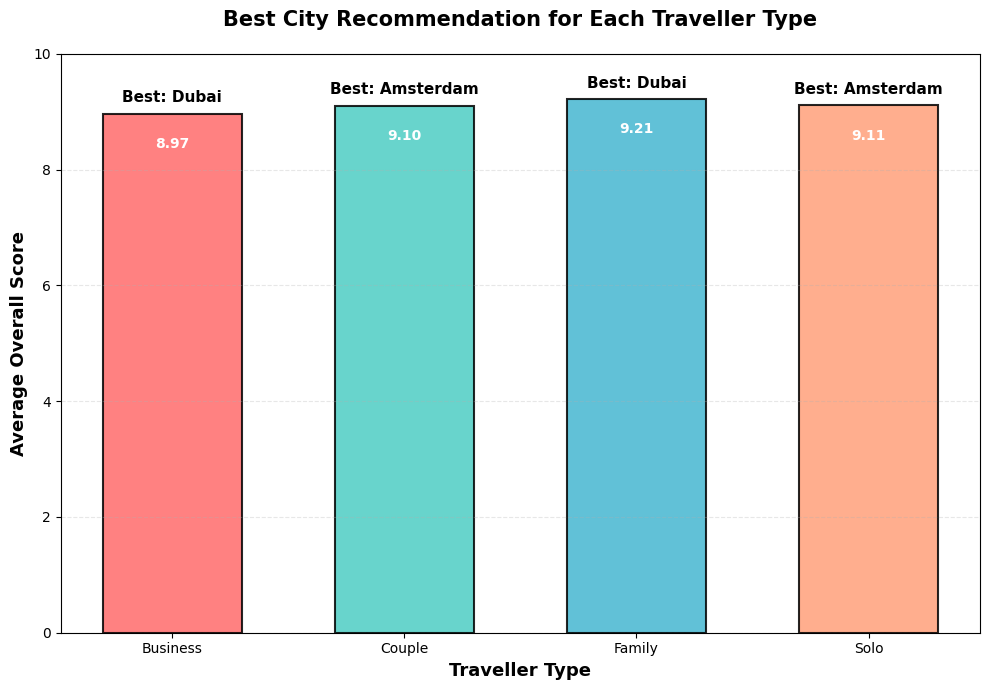
\includegraphics[keepaspectratio]{main_files/figure-pdf/cell-10-output-1.png}}

\section{Question 2}\label{question-2}

\subsubsection{🌍 Top Countries by Value-for-Money
Score}\label{top-countries-by-value-for-money-score}

This code calculates the \textbf{average value-for-money score} for each
country within every \textbf{age group}.\\
It then sorts the results and extracts the \textbf{top 3 countries} per
age group with the highest average scores.

\begin{Shaded}
\begin{Highlighting}[]
\NormalTok{top\_countries}\OperatorTok{=}\NormalTok{df.groupby([}\StringTok{"age\_group"}\NormalTok{,}\StringTok{"user\_country"}\NormalTok{])[}\StringTok{"score\_value\_for\_money"}\NormalTok{].mean().reset\_index()}
\NormalTok{top\_3}\OperatorTok{=}\NormalTok{top\_countries.sort\_values([}\StringTok{"age\_group"}\NormalTok{,}\StringTok{"score\_value\_for\_money"}\NormalTok{],ascending}\OperatorTok{=}\NormalTok{[}\VariableTok{True}\NormalTok{,}\VariableTok{False}\NormalTok{]).groupby(}\StringTok{"age\_group"}\NormalTok{).head(}\DecValTok{3}\NormalTok{)}
\BuiltInTok{print}\NormalTok{(top\_3)}
\end{Highlighting}
\end{Shaded}

\begin{verbatim}
    age_group user_country  score_value_for_money
5       18-24        Egypt               9.007317
19      18-24        Spain               8.768132
0       18-24    Argentina               8.689000
44      25-34        Spain               8.733259
43      25-34  South Korea               8.632800
37      25-34  Netherlands               8.542157
66      35-44    Singapore               8.795385
50      35-44    Argentina               8.696519
63      35-44  New Zealand               8.641079
94      45-54       Turkey               8.641778
89      45-54    Singapore               8.555914
79      45-54        China               8.547538
111       55+  New Zealand               8.686264
101       55+       Canada               8.621084
108       55+        Japan               8.524918
\end{verbatim}

\subsection{Plot of question 2}\label{plot-of-question-2}

\subsection{🌍 Top 3 Countries with Best Value-for-Money Score per Age
Group}\label{top-3-countries-with-best-value-for-money-score-per-age-group}

This chart illustrates which countries offer the best
``value-for-money'' as rated by different age groups. The y-axis shows
the average score, and the x-axis lists all countries that made it into
the top 3 for at least one age group.

\subsubsection{📊 Key Findings by Age
Group}\label{key-findings-by-age-group}

The top 3 countries for ``value-for-money'' vary significantly based on
the traveller's age:

\begin{itemize}
\tightlist
\item
  \textbf{Age Group 18-24 (Purple):}

  \begin{enumerate}
  \def\labelenumi{\arabic{enumi}.}
  \tightlist
  \item
    \textbf{Egypt} (Score: \textasciitilde9.0)
  \item
    \textbf{Spain} (Score: \textasciitilde8.8)
  \item
    \textbf{Argentina} (Score: \textasciitilde8.7)
  \end{enumerate}
\item
  \textbf{Age Group 25-34 (Teal):}

  \begin{enumerate}
  \def\labelenumi{\arabic{enumi}.}
  \tightlist
  \item
    \textbf{Spain} (Score: \textasciitilde8.8)
  \item
    \textbf{Singapore} (Score: \textasciitilde8.8)
  \item
    \textbf{Argentina} (Score: \textasciitilde8.7)
  \end{enumerate}
\item
  \textbf{Age Group 35-44 (Medium Green):}

  \begin{enumerate}
  \def\labelenumi{\arabic{enumi}.}
  \tightlist
  \item
    \textbf{Singapore} (Score: \textasciitilde8.6)
  \item
    \textbf{New Zealand} (Score: \textasciitilde8.6)
  \item
    \textbf{Turkey} (Score: \textasciitilde8.6)
  \end{enumerate}
\item
  \textbf{Age Group 45-54 (Light Green):}

  \begin{enumerate}
  \def\labelenumi{\arabic{enumi}.}
  \tightlist
  \item
    \textbf{New Zealand} (Score: \textasciitilde8.7)
  \item
    \textbf{Turkey} (Score: \textasciitilde8.6)
  \item
    \textbf{China} (Score: \textasciitilde8.5)
  \end{enumerate}
\item
  \textbf{Age Group 55+ (Yellow-Green):}

  \begin{enumerate}
  \def\labelenumi{\arabic{enumi}.}
  \tightlist
  \item
    \textbf{New Zealand} (Score: \textasciitilde8.7)
  \item
    \textbf{Canada} (Score: \textasciitilde8.6)
  \item
    \textbf{Japan} (Score: \textasciitilde6.9)
  \end{enumerate}
\end{itemize}

\subsubsection{Observations}\label{observations}

\begin{itemize}
\tightlist
\item
  \textbf{Cross-Generational Appeal:} \textbf{New Zealand} shows the
  broadest appeal, appearing in the top 3 for three different age groups
  (35-44, 45-54, and 55+). \textbf{Spain}, \textbf{Argentina},
  \textbf{Singapore}, and \textbf{Turkey} also appeal to multiple age
  groups.
\item
  \textbf{Unique Appeal:} \textbf{Egypt} is a top-3 country \emph{only}
  for the 18-24 age group. Similarly, \textbf{Canada} and \textbf{Japan}
  only appear in the top 3 for the 55+ group.
\item
  \textbf{Score Consistency:} Most top-rated countries have a very high
  score (above 8.5). The only exception is \textbf{Japan} for the 55+
  group, which has a noticeably lower score of \textasciitilde6.9.
\end{itemize}

\begin{Shaded}
\begin{Highlighting}[]
\NormalTok{plt.figure(figsize}\OperatorTok{=}\NormalTok{(}\DecValTok{10}\NormalTok{, }\DecValTok{6}\NormalTok{))}
\NormalTok{sns.barplot(}
\NormalTok{    data}\OperatorTok{=}\NormalTok{top\_3, }
\NormalTok{    x}\OperatorTok{=}\StringTok{\textquotesingle{}user\_country\textquotesingle{}}\NormalTok{, }
\NormalTok{    y}\OperatorTok{=}\StringTok{\textquotesingle{}score\_value\_for\_money\textquotesingle{}}\NormalTok{, }
\NormalTok{    hue}\OperatorTok{=}\StringTok{\textquotesingle{}age\_group\textquotesingle{}}\NormalTok{, }
\NormalTok{    palette}\OperatorTok{=}\StringTok{\textquotesingle{}viridis\textquotesingle{}}
\NormalTok{)}

\NormalTok{plt.title(}\StringTok{\textquotesingle{}Top 3 Countries with Best Value{-}for{-}Money Score per Age Group\textquotesingle{}}\NormalTok{, fontsize}\OperatorTok{=}\DecValTok{14}\NormalTok{, fontweight}\OperatorTok{=}\StringTok{\textquotesingle{}bold\textquotesingle{}}\NormalTok{)}
\NormalTok{plt.xlabel(}\StringTok{\textquotesingle{}Country\textquotesingle{}}\NormalTok{)}
\NormalTok{plt.ylabel(}\StringTok{\textquotesingle{}Average Value{-}for{-}Money Score\textquotesingle{}}\NormalTok{)}

\NormalTok{plt.legend(title}\OperatorTok{=}\StringTok{\textquotesingle{}Age Group\textquotesingle{}}\NormalTok{)}

\NormalTok{plt.tight\_layout()}
\NormalTok{plt.show()}
\end{Highlighting}
\end{Shaded}

\pandocbounded{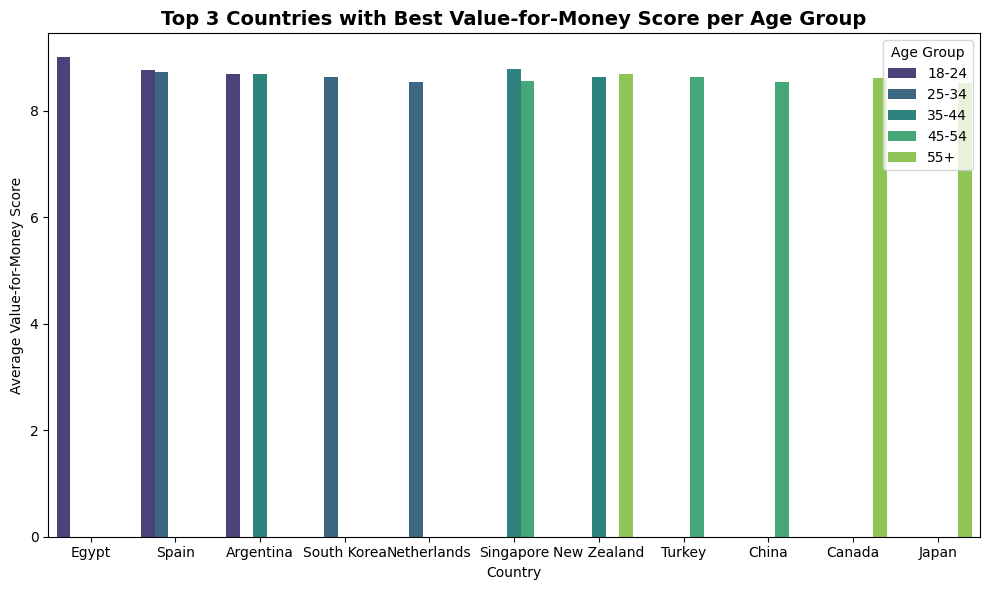
\includegraphics[keepaspectratio]{main_files/figure-pdf/cell-12-output-1.png}}

\section{---------------------------------------------------------}\label{section}

\begin{Shaded}
\begin{Highlighting}[]
\NormalTok{df.groupby(}\StringTok{\textquotesingle{}city\textquotesingle{}}\NormalTok{)[[}\StringTok{\textquotesingle{}country\_group\textquotesingle{}}\NormalTok{]].nunique()}
\end{Highlighting}
\end{Shaded}

\begin{longtable}[]{@{}ll@{}}
\toprule\noalign{}
& country\_group \\
city & \\
\midrule\noalign{}
\endhead
\bottomrule\noalign{}
\endlastfoot
Amsterdam & 1 \\
Bangkok & 1 \\
Barcelona & 1 \\
Berlin & 1 \\
Buenos Aires & 1 \\
Cairo & 1 \\
Cape Town & 1 \\
Dubai & 1 \\
Istanbul & 1 \\
Lagos & 1 \\
London & 1 \\
Mexico City & 1 \\
Moscow & 1 \\
Mumbai & 1 \\
New York & 1 \\
Paris & 1 \\
Rio de Janeiro & 1 \\
Rome & 1 \\
Seoul & 1 \\
Shanghai & 1 \\
Singapore & 1 \\
Sydney & 1 \\
Tokyo & 1 \\
Toronto & 1 \\
Wellington & 1 \\
\end{longtable}

\subsection{Encoding the user, gender , traveller type and
age}\label{encoding-the-user-gender-traveller-type-and-age}

\begin{Shaded}
\begin{Highlighting}[]
\NormalTok{df }\OperatorTok{=}\NormalTok{ pd.get\_dummies(df, columns}\OperatorTok{=}\NormalTok{[}\StringTok{\textquotesingle{}traveller\_type\textquotesingle{}}\NormalTok{], drop\_first}\OperatorTok{=}\VariableTok{True}\NormalTok{)}
\CommentTok{\# df = pd.get\_dummies(df, columns=[\textquotesingle{}user\_country\textquotesingle{}], drop\_first=True)}
\NormalTok{df }\OperatorTok{=}\NormalTok{ pd.get\_dummies(df, columns}\OperatorTok{=}\NormalTok{[}\StringTok{\textquotesingle{}user\_gender\textquotesingle{}}\NormalTok{], drop\_first}\OperatorTok{=}\VariableTok{True}\NormalTok{)}

\NormalTok{age\_order }\OperatorTok{=}\NormalTok{ \{}
    \StringTok{\textquotesingle{}18{-}24\textquotesingle{}}\NormalTok{: }\DecValTok{1}\NormalTok{,}
    \StringTok{\textquotesingle{}25{-}34\textquotesingle{}}\NormalTok{: }\DecValTok{2}\NormalTok{,}
    \StringTok{\textquotesingle{}35{-}44\textquotesingle{}}\NormalTok{: }\DecValTok{3}\NormalTok{,}
    \StringTok{\textquotesingle{}45{-}54\textquotesingle{}}\NormalTok{: }\DecValTok{4}\NormalTok{,}
    \StringTok{\textquotesingle{}55+\textquotesingle{}}\NormalTok{: }\DecValTok{5}
\NormalTok{\}}

\NormalTok{df[}\StringTok{\textquotesingle{}age\textquotesingle{}}\NormalTok{] }\OperatorTok{=}\NormalTok{ df[}\StringTok{\textquotesingle{}age\_group\textquotesingle{}}\NormalTok{].}\BuiltInTok{map}\NormalTok{(age\_order)}
\NormalTok{df.drop(columns}\OperatorTok{=}\NormalTok{[}\StringTok{\textquotesingle{}age\_group\textquotesingle{}}\NormalTok{], inplace}\OperatorTok{=}\VariableTok{True}\NormalTok{)}
\end{Highlighting}
\end{Shaded}

\begin{Shaded}
\begin{Highlighting}[]
\NormalTok{cols }\OperatorTok{=}\NormalTok{ [}
    \StringTok{\textquotesingle{}score\_cleanliness\textquotesingle{}}\NormalTok{, }\StringTok{\textquotesingle{}score\_facilities\textquotesingle{}}\NormalTok{, }\StringTok{\textquotesingle{}score\_staff\textquotesingle{}}\NormalTok{,}
    \StringTok{\textquotesingle{}star\_rating\textquotesingle{}}\NormalTok{, }\StringTok{\textquotesingle{}comfort\_base\textquotesingle{}}\NormalTok{, }\StringTok{\textquotesingle{}location\_base\textquotesingle{}}\NormalTok{,}
    \StringTok{\textquotesingle{}value\_for\_money\_base\textquotesingle{}}\NormalTok{, }\StringTok{\textquotesingle{}age\textquotesingle{}}

\NormalTok{]}

\NormalTok{corr }\OperatorTok{=}\NormalTok{ df[cols].corr()}

\ImportTok{import}\NormalTok{ seaborn }\ImportTok{as}\NormalTok{ sns}
\ImportTok{import}\NormalTok{ matplotlib.pyplot }\ImportTok{as}\NormalTok{ plt}

\NormalTok{plt.figure(figsize}\OperatorTok{=}\NormalTok{(}\DecValTok{8}\NormalTok{, }\DecValTok{6}\NormalTok{))}
\NormalTok{sns.heatmap(corr, annot}\OperatorTok{=}\VariableTok{True}\NormalTok{, cmap}\OperatorTok{=}\StringTok{\textquotesingle{}coolwarm\textquotesingle{}}\NormalTok{, center}\OperatorTok{=}\DecValTok{0}\NormalTok{)}
\NormalTok{plt.title(}\StringTok{"Correlation Heatmap (Simplified)"}\NormalTok{)}
\NormalTok{plt.show()}
\end{Highlighting}
\end{Shaded}

\pandocbounded{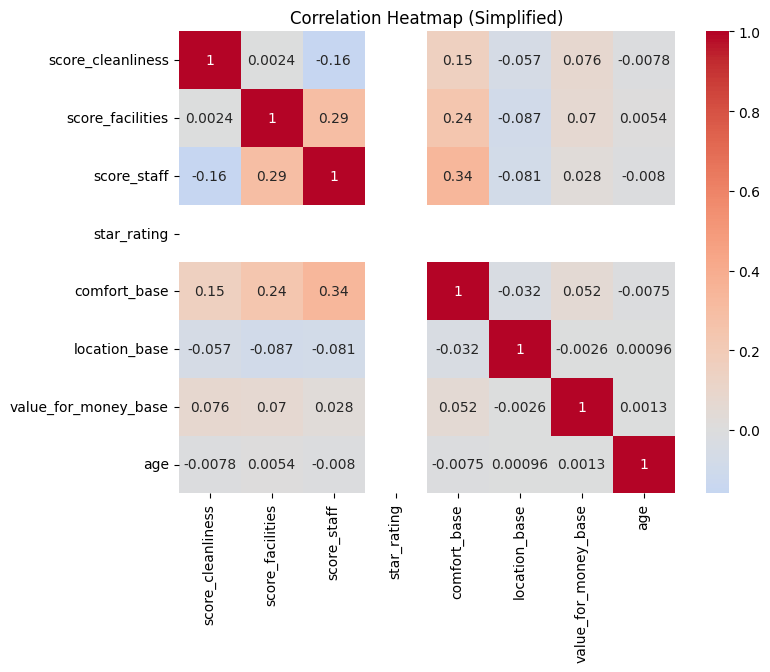
\includegraphics[keepaspectratio]{main_files/figure-pdf/cell-15-output-1.png}}

\begin{Shaded}
\begin{Highlighting}[]
\NormalTok{strong\_corr }\OperatorTok{=}\NormalTok{ corr[(corr }\OperatorTok{\textgreater{}} \DecValTok{0}\NormalTok{) }\OperatorTok{|}\NormalTok{ (corr }\OperatorTok{\textless{}=} \OperatorTok{{-}}\FloatTok{0.5}\NormalTok{)]}
\NormalTok{plt.figure(figsize}\OperatorTok{=}\NormalTok{(}\DecValTok{10}\NormalTok{, }\DecValTok{8}\NormalTok{))}
\NormalTok{sns.heatmap(strong\_corr, annot}\OperatorTok{=}\VariableTok{True}\NormalTok{, cmap}\OperatorTok{=}\StringTok{\textquotesingle{}coolwarm\textquotesingle{}}\NormalTok{, center}\OperatorTok{=}\DecValTok{0}\NormalTok{)}
\NormalTok{plt.title(}\StringTok{"Strong Correlations (\textgreater{}|0|)"}\NormalTok{)}
\NormalTok{plt.show()}
\end{Highlighting}
\end{Shaded}

\pandocbounded{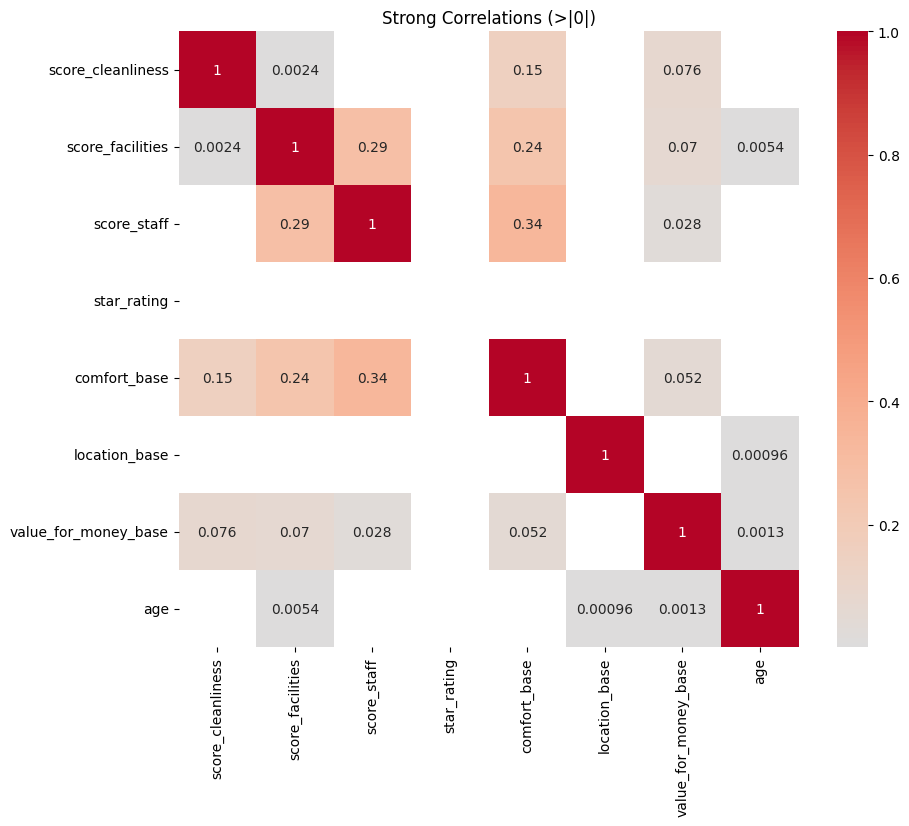
\includegraphics[keepaspectratio]{main_files/figure-pdf/cell-16-output-1.png}}

\subsection{Feature Engineering: Score
vs.~Baseline}\label{feature-engineering-score-vs.-baseline}

\subsubsection{📈 Creating ``Difference''
Features}\label{creating-difference-features}

This code block creates seven new ``difference'' (\texttt{diff\_})
columns.

These features are calculated by subtracting a ``base'' value from the
actual ``score'' for categories like cleanliness, comfort, and staff.
This measures how much a hotel \textbf{over-performs or under-performs}
compared to its baseline.

It also calculates the difference between the \texttt{score\_overall}
and the \texttt{star\_rating}, which can show if a hotel is rated higher
or lower than its official star category would suggest.

Finally, the code confirms the creation and prints the \texttt{head()}
of these new columns to show the results.

\begin{Shaded}
\begin{Highlighting}[]

\NormalTok{df[}\StringTok{\textquotesingle{}diff\_cleanliness\textquotesingle{}}\NormalTok{] }\OperatorTok{=}\NormalTok{ df[}\StringTok{\textquotesingle{}score\_cleanliness\textquotesingle{}}\NormalTok{] }\OperatorTok{{-}}\NormalTok{ df[}\StringTok{\textquotesingle{}cleanliness\_base\textquotesingle{}}\NormalTok{]}
\NormalTok{df[}\StringTok{\textquotesingle{}diff\_comfort\textquotesingle{}}\NormalTok{] }\OperatorTok{=}\NormalTok{ df[}\StringTok{\textquotesingle{}score\_comfort\textquotesingle{}}\NormalTok{] }\OperatorTok{{-}}\NormalTok{ df[}\StringTok{\textquotesingle{}comfort\_base\textquotesingle{}}\NormalTok{]}
\NormalTok{df[}\StringTok{\textquotesingle{}diff\_facilities\textquotesingle{}}\NormalTok{] }\OperatorTok{=}\NormalTok{ df[}\StringTok{\textquotesingle{}score\_facilities\textquotesingle{}}\NormalTok{] }\OperatorTok{{-}}\NormalTok{ df[}\StringTok{\textquotesingle{}facilities\_base\textquotesingle{}}\NormalTok{]}
\NormalTok{df[}\StringTok{\textquotesingle{}diff\_overall\_vs\_star\textquotesingle{}}\NormalTok{] }\OperatorTok{=}\NormalTok{ df[}\StringTok{\textquotesingle{}score\_overall\textquotesingle{}}\NormalTok{] }\OperatorTok{{-}}\NormalTok{ df[}\StringTok{\textquotesingle{}star\_rating\textquotesingle{}}\NormalTok{]}
\NormalTok{df[}\StringTok{\textquotesingle{}diff\_location\textquotesingle{}}\NormalTok{] }\OperatorTok{=}\NormalTok{ df[}\StringTok{\textquotesingle{}score\_location\textquotesingle{}}\NormalTok{] }\OperatorTok{{-}}\NormalTok{ df[}\StringTok{\textquotesingle{}location\_base\textquotesingle{}}\NormalTok{]}
\NormalTok{df[}\StringTok{\textquotesingle{}diff\_staff\textquotesingle{}}\NormalTok{] }\OperatorTok{=}\NormalTok{ df[}\StringTok{\textquotesingle{}score\_staff\textquotesingle{}}\NormalTok{] }\OperatorTok{{-}}\NormalTok{ df[}\StringTok{\textquotesingle{}staff\_base\textquotesingle{}}\NormalTok{]}
\NormalTok{df[}\StringTok{\textquotesingle{}diff\_value\_for\_money\textquotesingle{}}\NormalTok{] }\OperatorTok{=}\NormalTok{ df[}\StringTok{\textquotesingle{}score\_value\_for\_money\textquotesingle{}}\NormalTok{] }\OperatorTok{{-}}\NormalTok{ df[}\StringTok{\textquotesingle{}value\_for\_money\_base\textquotesingle{}}\NormalTok{]}

\BuiltInTok{print}\NormalTok{(}\StringTok{"Successfully created all \textquotesingle{}diff\textquotesingle{} features. ✅"}\NormalTok{)}
\BuiltInTok{print}\NormalTok{(}\StringTok{"}\CharTok{\textbackslash{}n}\StringTok{Head of the new \textquotesingle{}diff\textquotesingle{} features:"}\NormalTok{)}
\BuiltInTok{print}\NormalTok{(df[[ }\StringTok{\textquotesingle{}diff\_cleanliness\textquotesingle{}}\NormalTok{, }\StringTok{\textquotesingle{}diff\_comfort\textquotesingle{}}\NormalTok{, }\StringTok{\textquotesingle{}diff\_facilities\textquotesingle{}}\NormalTok{,}\StringTok{\textquotesingle{}diff\_overall\_vs\_star\textquotesingle{}}\NormalTok{, }\StringTok{\textquotesingle{}diff\_location\textquotesingle{}}\NormalTok{, }\StringTok{\textquotesingle{}diff\_staff\textquotesingle{}}\NormalTok{, }\StringTok{\textquotesingle{}diff\_value\_for\_money\textquotesingle{}}\NormalTok{]].head())}
\end{Highlighting}
\end{Shaded}

\begin{verbatim}
Successfully created all 'diff' features. ✅

Head of the new 'diff' features:
   diff_cleanliness  diff_comfort  diff_facilities  diff_overall_vs_star  \
0              -0.5          -0.1             -0.4                   3.7   
1               0.4           0.1             -0.3                   4.1   
2               0.9           0.1             -0.3                   3.8   
3              -0.2          -0.3             -0.4                   3.9   
4              -0.2           0.2              0.3                   4.1   

   diff_location  diff_staff  diff_value_for_money  
0           -0.5         0.2                   0.7  
1            0.1        -0.1                   0.4  
2           -0.4        -0.6                   0.2  
3           -0.1         0.1                  -0.5  
4           -0.7         0.3                   0.3  
\end{verbatim}

\subsubsection{🧹 Feature Selection and
Cleanup}\label{feature-selection-and-cleanup}

This cell removes unnecessary or non-numerical columns (like IDs, text,
and location data) that are not needed for analysis or modeling.\\
The resulting \texttt{final\_df} contains only the relevant features for
further processing.

\begin{Shaded}
\begin{Highlighting}[]

\ImportTok{from}\NormalTok{ typing }\ImportTok{import}\NormalTok{ final}


\NormalTok{columns\_to\_drop }\OperatorTok{=}\NormalTok{ [}
    \StringTok{\textquotesingle{}review\_id\textquotesingle{}}\NormalTok{,         }
    \StringTok{\textquotesingle{}user\_id\textquotesingle{}}\NormalTok{,           }
    \StringTok{\textquotesingle{}hotel\_id\textquotesingle{}}\NormalTok{,          }
    \StringTok{\textquotesingle{}review\_date\textquotesingle{}}\NormalTok{,      }
    \StringTok{\textquotesingle{}join\_date\textquotesingle{}}\NormalTok{,          }
    \StringTok{\textquotesingle{}review\_text\textquotesingle{}}\NormalTok{,       }
    \StringTok{\textquotesingle{}hotel\_name\textquotesingle{}}\NormalTok{,        }
    \StringTok{\textquotesingle{}hotel\_country\textquotesingle{}}\NormalTok{,   }
    \StringTok{\textquotesingle{}lat\textquotesingle{}}\NormalTok{, }
    \StringTok{\textquotesingle{}score\_overall\textquotesingle{}}\NormalTok{,}
    \StringTok{\textquotesingle{}score\_cleanliness\textquotesingle{}}\NormalTok{,}
    \StringTok{\textquotesingle{}score\_comfort\textquotesingle{}}\NormalTok{,}
    \StringTok{\textquotesingle{}score\_facilities\textquotesingle{}}\NormalTok{,}
    \StringTok{\textquotesingle{}score\_location\textquotesingle{}}\NormalTok{,}
    \StringTok{\textquotesingle{}score\_staff\textquotesingle{}}\NormalTok{,}
    \StringTok{\textquotesingle{}score\_value\_for\_money\textquotesingle{}}\NormalTok{,}
    \StringTok{\textquotesingle{}city\textquotesingle{}}\NormalTok{,}
    \StringTok{\textquotesingle{}star\_rating\textquotesingle{}}\NormalTok{,}
    \StringTok{\textquotesingle{}cleanliness\_base\textquotesingle{}}\NormalTok{,}
    \StringTok{\textquotesingle{}comfort\_base\textquotesingle{}}\NormalTok{,}
    \StringTok{\textquotesingle{}facilities\_base\textquotesingle{}}\NormalTok{,}
    \StringTok{\textquotesingle{}location\_base\textquotesingle{}}\NormalTok{,}
    \StringTok{\textquotesingle{}staff\_base\textquotesingle{}}\NormalTok{,}
    \StringTok{\textquotesingle{}value\_for\_money\_base\textquotesingle{}}\NormalTok{,   }
    \StringTok{\textquotesingle{}user\_country\textquotesingle{}}\NormalTok{,            }
    \StringTok{\textquotesingle{}lon\textquotesingle{}}  
\NormalTok{]}
\NormalTok{final\_df}\OperatorTok{=}\NormalTok{df.drop(columns}\OperatorTok{=}\NormalTok{columns\_to\_drop)}

\CommentTok{\# final\_df.to\_csv(\textquotesingle{}final\_dataset.csv\textquotesingle{}, index=False)   }
\NormalTok{final\_df.head()}
\end{Highlighting}
\end{Shaded}

\begin{longtable}[]{@{}lllllllllllllll@{}}
\toprule\noalign{}
& country\_group & traveller\_type\_Couple & traveller\_type\_Family &
traveller\_type\_Solo & user\_gender\_Male & user\_gender\_Other & age &
diff\_cleanliness & diff\_comfort & diff\_facilities &
diff\_overall\_vs\_star & diff\_location & diff\_staff &
diff\_value\_for\_money \\
\midrule\noalign{}
\endhead
\bottomrule\noalign{}
\endlastfoot
0 & North\_America & False & False & True & False & False & 2 & -0.5 &
-0.1 & -0.4 & 3.7 & -0.5 & 0.2 & 0.7 \\
1 & East\_Asia & True & False & False & False & False & 3 & 0.4 & 0.1 &
-0.3 & 4.1 & 0.1 & -0.1 & 0.4 \\
2 & Africa & True & False & False & False & False & 5 & 0.9 & 0.1 & -0.3
& 3.8 & -0.4 & -0.6 & 0.2 \\
3 & Western\_Europe & False & False & False & False & False & 3 & -0.2 &
-0.3 & -0.4 & 3.9 & -0.1 & 0.1 & -0.5 \\
4 & Eastern\_Europe & False & True & False & True & False & 4 & -0.2 &
0.2 & 0.3 & 4.1 & -0.7 & 0.3 & 0.3 \\
\end{longtable}

\begin{Shaded}
\begin{Highlighting}[]
\NormalTok{final\_df.info()}
\end{Highlighting}
\end{Shaded}

\begin{verbatim}
<class 'pandas.core.frame.DataFrame'>
RangeIndex: 50000 entries, 0 to 49999
Data columns (total 14 columns):
 #   Column                 Non-Null Count  Dtype  
---  ------                 --------------  -----  
 0   country_group          50000 non-null  object 
 1   traveller_type_Couple  50000 non-null  bool   
 2   traveller_type_Family  50000 non-null  bool   
 3   traveller_type_Solo    50000 non-null  bool   
 4   user_gender_Male       50000 non-null  bool   
 5   user_gender_Other      50000 non-null  bool   
 6   age                    50000 non-null  int64  
 7   diff_cleanliness       50000 non-null  float64
 8   diff_comfort           50000 non-null  float64
 9   diff_facilities        50000 non-null  float64
 10  diff_overall_vs_star   50000 non-null  float64
 11  diff_location          50000 non-null  float64
 12  diff_staff             50000 non-null  float64
 13  diff_value_for_money   50000 non-null  float64
dtypes: bool(5), float64(7), int64(1), object(1)
memory usage: 3.7+ MB
\end{verbatim}

\begin{Shaded}
\begin{Highlighting}[]
\NormalTok{final\_df.to\_csv(}\StringTok{\textquotesingle{}final\_dataset.csv\textquotesingle{}}\NormalTok{, index}\OperatorTok{=}\VariableTok{False}\NormalTok{)}
\end{Highlighting}
\end{Shaded}

\section{Checking for null values}\label{checking-for-null-values}

after checking the data in the table there was no null values

\begin{Shaded}
\begin{Highlighting}[]
\NormalTok{final\_df.isnull().}\BuiltInTok{sum}\NormalTok{()}
\end{Highlighting}
\end{Shaded}

\begin{verbatim}
country_group            0
traveller_type_Couple    0
traveller_type_Family    0
traveller_type_Solo      0
user_gender_Male         0
user_gender_Other        0
age                      0
diff_cleanliness         0
diff_comfort             0
diff_facilities          0
diff_overall_vs_star     0
diff_location            0
diff_staff               0
diff_value_for_money     0
dtype: int64
\end{verbatim}

\begin{Shaded}
\begin{Highlighting}[]
\NormalTok{final\_df.to\_csv(}\StringTok{\textquotesingle{}final\_dataset.csv\textquotesingle{}}\NormalTok{, index}\OperatorTok{=}\VariableTok{False}\NormalTok{)}
\end{Highlighting}
\end{Shaded}

\subsection{🎯 Defining Features (X) and Target
(y)}\label{defining-features-x-and-target-y}

This code block prepares the data for a machine learning model by
separating it into two distinct variables:

\begin{enumerate}
\def\labelenumi{\arabic{enumi}.}
\tightlist
\item
  \textbf{\texttt{X} (Features)}: This DataFrame, \texttt{X}, holds all
  the \textbf{independent variables} (or features) that the model will
  use to learn and make predictions. It is created by selecting specific
  columns from the \texttt{final\_df}, including:

  \begin{itemize}
  \tightlist
  \item
    The \textbf{``difference'' features} (e.g.,
    \texttt{diff\_overall\_vs\_star}, \texttt{diff\_cleanliness}).
  \item
    \textbf{One-hot encoded features} for \texttt{traveller\_type} and
    \texttt{user\_gender}.
  \item
    The numerical \texttt{age} feature.
  \end{itemize}
\item
  \textbf{\texttt{y} (Target)}: This pandas Series, \texttt{y}, holds
  the \textbf{dependent variable} (or target) that the model will be
  trained to predict.

  \begin{itemize}
  \tightlist
  \item
    In this case, the target is the \texttt{country\_group} column.
  \end{itemize}
\end{enumerate}

\begin{Shaded}
\begin{Highlighting}[]
\NormalTok{X }\OperatorTok{=}\NormalTok{ final\_df[[}\StringTok{\textquotesingle{}diff\_overall\_vs\_star\textquotesingle{}}\NormalTok{,}\StringTok{\textquotesingle{}diff\_cleanliness\textquotesingle{}}\NormalTok{,}\StringTok{\textquotesingle{}diff\_comfort\textquotesingle{}}\NormalTok{,}\StringTok{\textquotesingle{}diff\_facilities\textquotesingle{}}\NormalTok{,}\StringTok{\textquotesingle{}diff\_location\textquotesingle{}}\NormalTok{,}\StringTok{\textquotesingle{}diff\_staff\textquotesingle{}}\NormalTok{,}\StringTok{\textquotesingle{}diff\_value\_for\_money\textquotesingle{}}\NormalTok{,}\StringTok{\textquotesingle{}traveller\_type\_Couple\textquotesingle{}}\NormalTok{,}\StringTok{\textquotesingle{}traveller\_type\_Family\textquotesingle{}}\NormalTok{,}\StringTok{\textquotesingle{}traveller\_type\_Solo\textquotesingle{}}\NormalTok{, }\StringTok{\textquotesingle{}user\_gender\_Male\textquotesingle{}}\NormalTok{,}\StringTok{\textquotesingle{}user\_gender\_Other\textquotesingle{}}\NormalTok{,}\StringTok{\textquotesingle{}age\textquotesingle{}}\NormalTok{ ]] }
\NormalTok{y }\OperatorTok{=}\NormalTok{ final\_df[}\StringTok{\textquotesingle{}country\_group\textquotesingle{}}\NormalTok{]}
\end{Highlighting}
\end{Shaded}

\subsection{Plot: Target Variable
Distribution}\label{plot-target-variable-distribution}

\subsubsection{📊 Country Group
Distribution}\label{country-group-distribution}

This line of code visualizes the distribution of the target variable
\texttt{y} (which contains the ``Country Group'' categories).

It first performs a \texttt{value\_counts()} to count the total number
of occurrences for each unique category in \texttt{y}. Then, it
immediately uses
\texttt{.plot(kind=\textquotesingle{}bar\textquotesingle{})} to create a
\textbf{bar chart} of these counts. The \texttt{title} is set to
``Country Group Distribution'', and \texttt{plt.show()} displays the
final visual.

\textbf{Observation:} The plot shows an imbalanced distribution, with a
\textbf{significantly larger number of samples for the ``Western
Europe'' category} compared to the others.

\begin{Shaded}
\begin{Highlighting}[]
\NormalTok{y.value\_counts().plot(kind}\OperatorTok{=}\StringTok{\textquotesingle{}bar\textquotesingle{}}\NormalTok{, title}\OperatorTok{=}\StringTok{\textquotesingle{}Country Group Distribution\textquotesingle{}}\NormalTok{)}
\NormalTok{plt.show()}
\end{Highlighting}
\end{Shaded}

\pandocbounded{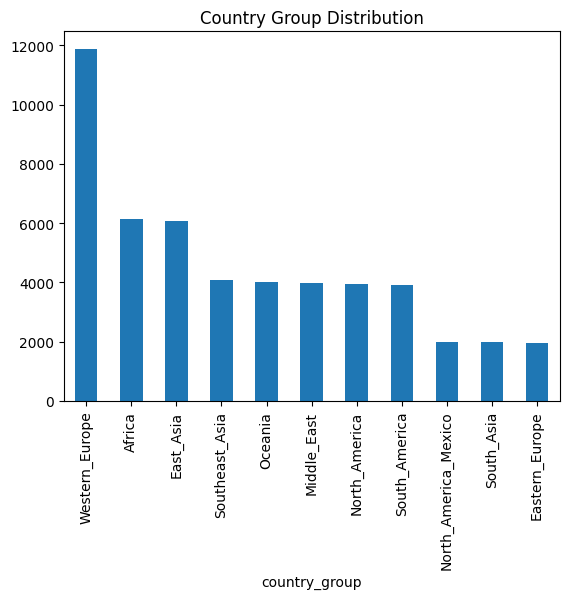
\includegraphics[keepaspectratio]{main_files/figure-pdf/cell-24-output-1.png}}

\subsection{Data Preparation}\label{data-preparation}

\subsubsection{🔪 Splitting Data into Training and Test
Sets}\label{splitting-data-into-training-and-test-sets}

This line of code uses the \texttt{train\_test\_split} function from
scikit-learn to divide the dataset into two parts: a \textbf{training
set} and a \textbf{test set}.

\begin{itemize}
\tightlist
\item
  \textbf{\texttt{X,\ y}}: These are the complete datasets, with
  \texttt{X} being the features and \texttt{y} being the target variable
  (labels).
\item
  \textbf{\texttt{test\_size=0.2}}: This parameter specifies that
  \textbf{20\%} of the data should be reserved for the test set. The
  remaining \textbf{80\%} will be used for the training set.
\item
  \textbf{\texttt{random\_state=42}}: This acts as a seed for the random
  shuffling. By setting a specific number (like 42), we ensure that the
  split is \textbf{reproducible}---meaning, every time this code is run,
  the data will be split in the exact same way.
\end{itemize}

The function returns four new variables: 1. \textbf{\texttt{X\_train}}:
The 80\% of features used for training the model. 2.
\textbf{\texttt{X\_test}}: The 20\% of features used for testing the
model. 3. \textbf{\texttt{y\_train}}: The corresponding 80\% of labels
for training. 4. \textbf{\texttt{y\_test}}: The corresponding 20\% of
labels for testing.

\begin{Shaded}
\begin{Highlighting}[]
\NormalTok{X\_train, X\_test, y\_train, y\_test }\OperatorTok{=}\NormalTok{ train\_test\_split(X, y, test\_size}\OperatorTok{=}\FloatTok{0.2}\NormalTok{, random\_state}\OperatorTok{=}\DecValTok{42}\NormalTok{)}
\end{Highlighting}
\end{Shaded}

\begin{Shaded}
\begin{Highlighting}[]
\NormalTok{log\_model }\OperatorTok{=}\NormalTok{ LogisticRegression(}
\NormalTok{    max\_iter}\OperatorTok{=}\DecValTok{100}\NormalTok{,}
\NormalTok{)}
\end{Highlighting}
\end{Shaded}

\begin{Shaded}
\begin{Highlighting}[]
\NormalTok{log\_model.fit(X\_train,y\_train)}
\end{Highlighting}
\end{Shaded}

\begin{verbatim}
c:\Users\abdel\fire_env_tf\lib\site-packages\sklearn\linear_model\_logistic.py:473: ConvergenceWarning: lbfgs failed to converge after 100 iteration(s) (status=1):
STOP: TOTAL NO. OF ITERATIONS REACHED LIMIT

Increase the number of iterations to improve the convergence (max_iter=100).
You might also want to scale the data as shown in:
    https://scikit-learn.org/stable/modules/preprocessing.html
Please also refer to the documentation for alternative solver options:
    https://scikit-learn.org/stable/modules/linear_model.html#logistic-regression
  n_iter_i = _check_optimize_result(
\end{verbatim}

\begin{longtable}[]{@{}lll@{}}
\toprule\noalign{}
\endhead
\bottomrule\noalign{}
\endlastfoot
\emph{} & penalty~ & \textquotesingle l2\textquotesingle{} \\
\emph{} & dual~ & False \\
\emph{} & tol~ & 0.0001 \\
\emph{} & C~ & 1.0 \\
\emph{} & fit\_intercept~ & True \\
\emph{} & intercept\_scaling~ & 1 \\
\emph{} & class\_weight~ & None \\
\emph{} & random\_state~ & None \\
\emph{} & solver~ & \textquotesingle lbfgs\textquotesingle{} \\
\emph{} & max\_iter~ & 100 \\
\emph{} & multi\_class~ &
\textquotesingle deprecated\textquotesingle{} \\
\emph{} & verbose~ & 0 \\
\emph{} & warm\_start~ & False \\
\emph{} & n\_jobs~ & None \\
\emph{} & l1\_ratio~ & None \\
\end{longtable}

\begin{Shaded}
\begin{Highlighting}[]
\NormalTok{y\_pred }\OperatorTok{=}\NormalTok{ log\_model.predict(X\_test)}

\BuiltInTok{print}\NormalTok{(}\StringTok{"=== Logistic Regression Evaluation ==="}\NormalTok{)}
\BuiltInTok{print}\NormalTok{(}\StringTok{"Accuracy:"}\NormalTok{, accuracy\_score(y\_test, y\_pred))}
\BuiltInTok{print}\NormalTok{(}\StringTok{"Precision:"}\NormalTok{, precision\_score(y\_test, y\_pred, average}\OperatorTok{=}\StringTok{\textquotesingle{}weighted\textquotesingle{}}\NormalTok{))}
\BuiltInTok{print}\NormalTok{(}\StringTok{"Recall:"}\NormalTok{, recall\_score(y\_test, y\_pred, average}\OperatorTok{=}\StringTok{\textquotesingle{}weighted\textquotesingle{}}\NormalTok{))}
\BuiltInTok{print}\NormalTok{(}\StringTok{"F1 Score:"}\NormalTok{, f1\_score(y\_test, y\_pred, average}\OperatorTok{=}\StringTok{\textquotesingle{}weighted\textquotesingle{}}\NormalTok{))}
\BuiltInTok{print}\NormalTok{(}\StringTok{"}\CharTok{\textbackslash{}n}\StringTok{Detailed Report:}\CharTok{\textbackslash{}n}\StringTok{"}\NormalTok{, classification\_report(y\_test, y\_pred))}
\end{Highlighting}
\end{Shaded}

\begin{verbatim}
=== Logistic Regression Evaluation ===
Accuracy: 0.3222
Precision: 0.24346349673260093
Recall: 0.3222
F1 Score: 0.2348494413158195

Detailed Report:
                       precision    recall  f1-score   support

              Africa       0.33      0.64      0.44      1247
           East_Asia       0.29      0.29      0.29      1195
      Eastern_Europe       0.00      0.00      0.00       358
         Middle_East       0.08      0.00      0.01       816
       North_America       0.21      0.02      0.04       776
North_America_Mexico       0.08      0.03      0.05       400
             Oceania       0.17      0.00      0.00       805
       South_America       0.41      0.14      0.21       813
          South_Asia       0.00      0.00      0.00       389
      Southeast_Asia       0.15      0.08      0.11       818
      Western_Europe       0.35      0.78      0.48      2383

            accuracy                           0.32     10000
           macro avg       0.19      0.18      0.15     10000
        weighted avg       0.24      0.32      0.23     10000
\end{verbatim}

\begin{verbatim}
c:\Users\abdel\fire_env_tf\lib\site-packages\sklearn\metrics\_classification.py:1731: UndefinedMetricWarning: Precision is ill-defined and being set to 0.0 in labels with no predicted samples. Use `zero_division` parameter to control this behavior.
  _warn_prf(average, modifier, f"{metric.capitalize()} is", result.shape[0])
c:\Users\abdel\fire_env_tf\lib\site-packages\sklearn\metrics\_classification.py:1731: UndefinedMetricWarning: Precision is ill-defined and being set to 0.0 in labels with no predicted samples. Use `zero_division` parameter to control this behavior.
  _warn_prf(average, modifier, f"{metric.capitalize()} is", result.shape[0])
c:\Users\abdel\fire_env_tf\lib\site-packages\sklearn\metrics\_classification.py:1731: UndefinedMetricWarning: Precision is ill-defined and being set to 0.0 in labels with no predicted samples. Use `zero_division` parameter to control this behavior.
  _warn_prf(average, modifier, f"{metric.capitalize()} is", result.shape[0])
c:\Users\abdel\fire_env_tf\lib\site-packages\sklearn\metrics\_classification.py:1731: UndefinedMetricWarning: Precision is ill-defined and being set to 0.0 in labels with no predicted samples. Use `zero_division` parameter to control this behavior.
  _warn_prf(average, modifier, f"{metric.capitalize()} is", result.shape[0])
\end{verbatim}

\begin{Shaded}
\begin{Highlighting}[]
\NormalTok{final\_df.info()}
\end{Highlighting}
\end{Shaded}

\begin{verbatim}
<class 'pandas.core.frame.DataFrame'>
RangeIndex: 50000 entries, 0 to 49999
Data columns (total 14 columns):
 #   Column                 Non-Null Count  Dtype  
---  ------                 --------------  -----  
 0   country_group          50000 non-null  object 
 1   traveller_type_Couple  50000 non-null  bool   
 2   traveller_type_Family  50000 non-null  bool   
 3   traveller_type_Solo    50000 non-null  bool   
 4   user_gender_Male       50000 non-null  bool   
 5   user_gender_Other      50000 non-null  bool   
 6   age                    50000 non-null  int64  
 7   diff_cleanliness       50000 non-null  float64
 8   diff_comfort           50000 non-null  float64
 9   diff_facilities        50000 non-null  float64
 10  diff_overall_vs_star   50000 non-null  float64
 11  diff_location          50000 non-null  float64
 12  diff_staff             50000 non-null  float64
 13  diff_value_for_money   50000 non-null  float64
dtypes: bool(5), float64(7), int64(1), object(1)
memory usage: 3.7+ MB
\end{verbatim}

\begin{Shaded}
\begin{Highlighting}[]
\CommentTok{\# global explanation}
\NormalTok{explainer }\OperatorTok{=}\NormalTok{ shap.LinearExplainer(log\_model, X\_train)}

\NormalTok{shap\_values }\OperatorTok{=}\NormalTok{ explainer.shap\_values(X\_test)}

\ControlFlowTok{if} \BuiltInTok{isinstance}\NormalTok{(shap\_values, }\BuiltInTok{list}\NormalTok{):}
\NormalTok{    shap\_values }\OperatorTok{=}\NormalTok{ shap\_values[}\DecValTok{1}\NormalTok{] }\ControlFlowTok{if} \BuiltInTok{len}\NormalTok{(shap\_values) }\OperatorTok{\textgreater{}} \DecValTok{1} \ControlFlowTok{else}\NormalTok{ shap\_values[}\DecValTok{0}\NormalTok{]}


\NormalTok{shap\_values }\OperatorTok{=}\NormalTok{ np.array(shap\_values, dtype}\OperatorTok{=}\NormalTok{np.float64)}


\NormalTok{shap.summary\_plot(shap\_values, X\_test, plot\_type}\OperatorTok{=}\StringTok{"bar"}\NormalTok{, max\_display}\OperatorTok{=}\NormalTok{X\_test.shape[}\DecValTok{1}\NormalTok{], show}\OperatorTok{=}\VariableTok{True}\NormalTok{)}
\NormalTok{shap.summary\_plot(shap\_values, X\_test)}
\end{Highlighting}
\end{Shaded}

\pandocbounded{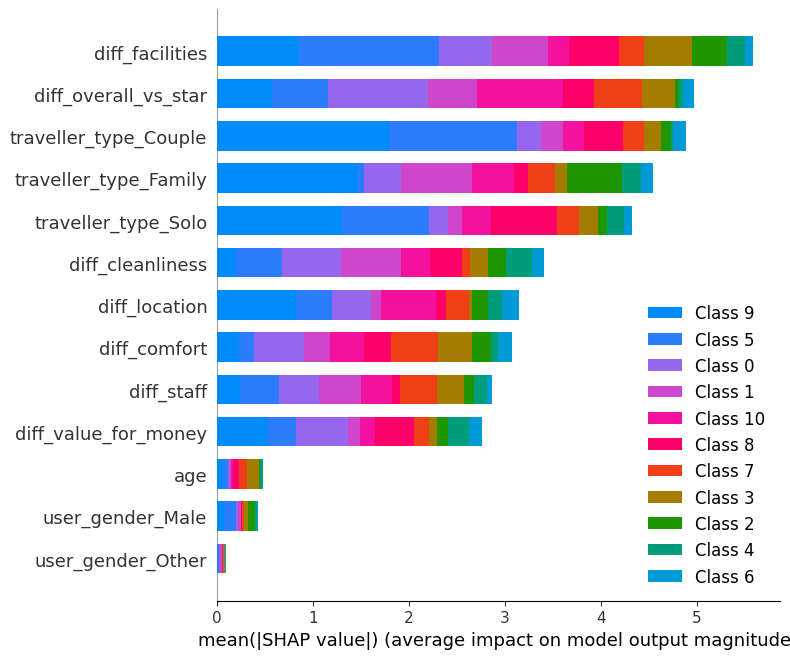
\includegraphics[keepaspectratio]{main_files/figure-pdf/cell-30-output-1.png}}

\pandocbounded{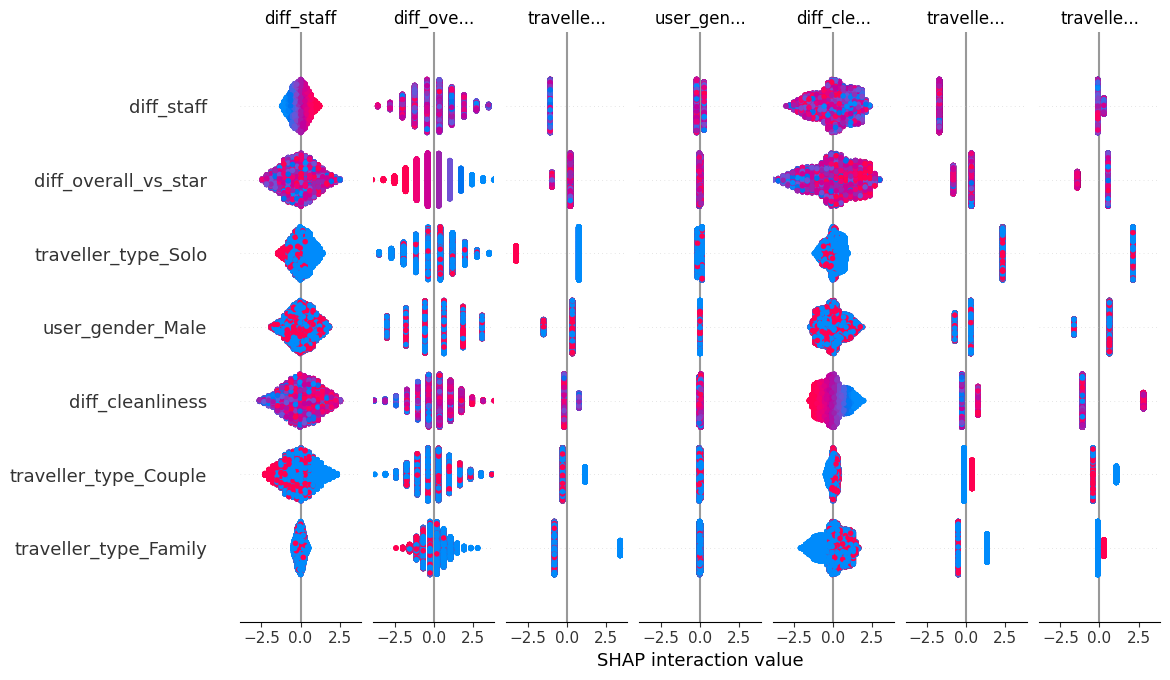
\includegraphics[keepaspectratio]{main_files/figure-pdf/cell-30-output-2.png}}

\begin{Shaded}
\begin{Highlighting}[]
\NormalTok{scaler }\OperatorTok{=}\NormalTok{ StandardScaler()}
\NormalTok{X\_train\_scaled }\OperatorTok{=}\NormalTok{ scaler.fit\_transform(X\_train)}
\NormalTok{X\_test\_scaled }\OperatorTok{=}\NormalTok{ scaler.transform(X\_test)}
\end{Highlighting}
\end{Shaded}

\begin{Shaded}
\begin{Highlighting}[]
\CommentTok{\# Ensure consistent random state}
\NormalTok{np.random.seed(}\DecValTok{42}\NormalTok{)}

\BuiltInTok{print}\NormalTok{(}\StringTok{"Train shape:"}\NormalTok{, X\_train.shape)}
\BuiltInTok{print}\NormalTok{(}\StringTok{"Test shape:"}\NormalTok{, X\_test.shape)}

\NormalTok{explainer }\OperatorTok{=}\NormalTok{ LimeTabularExplainer(}
\NormalTok{    training\_data}\OperatorTok{=}\NormalTok{np.array(X\_train),}
\NormalTok{    feature\_names}\OperatorTok{=}\NormalTok{X\_train.columns,}
\NormalTok{    class\_names}\OperatorTok{=}\NormalTok{log\_model.classes\_.astype(}\BuiltInTok{str}\NormalTok{),}
\NormalTok{    mode}\OperatorTok{=}\StringTok{\textquotesingle{}classification\textquotesingle{}}\NormalTok{,}
\NormalTok{    discretize\_continuous}\OperatorTok{=}\VariableTok{True}
\NormalTok{)}

\NormalTok{sample\_idx }\OperatorTok{=} \DecValTok{39}
\NormalTok{sample }\OperatorTok{=}\NormalTok{ X\_test.iloc[sample\_idx]}


\NormalTok{pred\_label }\OperatorTok{=}\NormalTok{ log\_model.predict(sample.values.reshape(}\DecValTok{1}\NormalTok{, }\OperatorTok{{-}}\DecValTok{1}\NormalTok{))[}\DecValTok{0}\NormalTok{]      }
\NormalTok{pred\_class\_idx }\OperatorTok{=}\NormalTok{ np.where(log\_model.classes\_ }\OperatorTok{==}\NormalTok{ pred\_label)[}\DecValTok{0}\NormalTok{][}\DecValTok{0}\NormalTok{]    }
\NormalTok{pred\_class\_name }\OperatorTok{=}\NormalTok{ log\_model.classes\_[pred\_class\_idx]}

\BuiltInTok{print}\NormalTok{(}\SpecialStringTok{f"Predicted class: }\SpecialCharTok{\{}\NormalTok{pred\_class\_name}\SpecialCharTok{\}}\SpecialStringTok{"}\NormalTok{)}


\NormalTok{exp }\OperatorTok{=}\NormalTok{ explainer.explain\_instance(}
\NormalTok{    data\_row}\OperatorTok{=}\NormalTok{sample,}
\NormalTok{    predict\_fn}\OperatorTok{=}\NormalTok{log\_model.predict\_proba, }
\NormalTok{    num\_features}\OperatorTok{=}\DecValTok{10}\NormalTok{,}
\NormalTok{    labels}\OperatorTok{=}\NormalTok{[pred\_class\_idx]   }
\NormalTok{)}

\NormalTok{exp.show\_in\_notebook(show\_table}\OperatorTok{=}\VariableTok{True}\NormalTok{, labels}\OperatorTok{=}\NormalTok{[pred\_class\_idx])}

\BuiltInTok{print}\NormalTok{(}\SpecialStringTok{f"}\CharTok{\textbackslash{}n}\SpecialStringTok{LIME Explanation for predicted class \textquotesingle{}}\SpecialCharTok{\{}\NormalTok{pred\_class\_name}\SpecialCharTok{\}}\SpecialStringTok{\textquotesingle{}:"}\NormalTok{)}
\ControlFlowTok{for}\NormalTok{ feature, weight }\KeywordTok{in}\NormalTok{ exp.as\_list(label}\OperatorTok{=}\NormalTok{pred\_class\_idx):}
    \BuiltInTok{print}\NormalTok{(}\SpecialStringTok{f"}\SpecialCharTok{\{}\NormalTok{feature}\SpecialCharTok{\}}\SpecialStringTok{: }\SpecialCharTok{\{}\NormalTok{weight}\SpecialCharTok{:.4f\}}\SpecialStringTok{"}\NormalTok{)}
\end{Highlighting}
\end{Shaded}

\begin{verbatim}
Train shape: (40000, 13)
Test shape: (10000, 13)
\end{verbatim}

\begin{verbatim}
c:\Users\abdel\fire_env_tf\lib\site-packages\sklearn\utils\validation.py:2749: UserWarning: X does not have valid feature names, but LogisticRegression was fitted with feature names
  warnings.warn(
c:\Users\abdel\fire_env_tf\lib\site-packages\lime\discretize.py:110: FutureWarning: Series.__getitem__ treating keys as positions is deprecated. In a future version, integer keys will always be treated as labels (consistent with DataFrame behavior). To access a value by position, use `ser.iloc[pos]`
  ret[feature] = int(self.lambdas[feature](ret[feature]))
c:\Users\abdel\fire_env_tf\lib\site-packages\lime\discretize.py:110: FutureWarning: Series.__setitem__ treating keys as positions is deprecated. In a future version, integer keys will always be treated as labels (consistent with DataFrame behavior). To set a value by position, use `ser.iloc[pos] = value`
  ret[feature] = int(self.lambdas[feature](ret[feature]))
c:\Users\abdel\fire_env_tf\lib\site-packages\lime\lime_tabular.py:544: FutureWarning: Series.__getitem__ treating keys as positions is deprecated. In a future version, integer keys will always be treated as labels (consistent with DataFrame behavior). To access a value by position, use `ser.iloc[pos]`
  binary_column = (inverse_column == first_row[column]).astype(int)
c:\Users\abdel\fire_env_tf\lib\site-packages\sklearn\utils\validation.py:2749: UserWarning: X does not have valid feature names, but LogisticRegression was fitted with feature names
  warnings.warn(
c:\Users\abdel\fire_env_tf\lib\site-packages\lime\discretize.py:110: FutureWarning: Series.__getitem__ treating keys as positions is deprecated. In a future version, integer keys will always be treated as labels (consistent with DataFrame behavior). To access a value by position, use `ser.iloc[pos]`
  ret[feature] = int(self.lambdas[feature](ret[feature]))
c:\Users\abdel\fire_env_tf\lib\site-packages\lime\discretize.py:110: FutureWarning: Series.__setitem__ treating keys as positions is deprecated. In a future version, integer keys will always be treated as labels (consistent with DataFrame behavior). To set a value by position, use `ser.iloc[pos] = value`
  ret[feature] = int(self.lambdas[feature](ret[feature]))
c:\Users\abdel\fire_env_tf\lib\site-packages\lime\lime_tabular.py:427: FutureWarning: Series.__getitem__ treating keys as positions is deprecated. In a future version, integer keys will always be treated as labels (consistent with DataFrame behavior). To access a value by position, use `ser.iloc[pos]`
  discretized_instance[f])]
\end{verbatim}

\begin{verbatim}
Predicted class: Western_Europe
\end{verbatim}

\begin{verbatim}
<IPython.core.display.HTML object>
\end{verbatim}

\begin{verbatim}

LIME Explanation for predicted class 'Western_Europe':
diff_overall_vs_star <= 3.80: -0.1643
traveller_type_Family <= 0.00: 0.1021
diff_location <= -0.40: 0.0948
diff_staff <= -0.30: 0.0415
traveller_type_Solo <= 0.00: 0.0371
0.00 < diff_value_for_money <= 0.30: -0.0312
0.00 < diff_comfort <= 0.20: -0.0236
0.00 < traveller_type_Couple <= 1.00: 0.0162
-0.40 < diff_cleanliness <= 0.00: 0.0161
age > 4.00: 0.0115
\end{verbatim}

\subsubsection{Encoded the string labels into integers and converted
them into one-hot vectors so the neural network can understand and
process the target classes numerically during
training.}\label{encoded-the-string-labels-into-integers-and-converted-them-into-one-hot-vectors-so-the-neural-network-can-understand-and-process-the-target-classes-numerically-during-training.}

\begin{Shaded}
\begin{Highlighting}[]
\CommentTok{\# Encode string labels into integers}
\NormalTok{le }\OperatorTok{=}\NormalTok{ LabelEncoder()}
\NormalTok{y\_encoded }\OperatorTok{=}\NormalTok{ le.fit\_transform(y)}

\CommentTok{\# One{-}hot encode for NN output layer}
\NormalTok{y\_categorical }\OperatorTok{=}\NormalTok{ to\_categorical(y\_encoded)}
\end{Highlighting}
\end{Shaded}

\begin{Shaded}
\begin{Highlighting}[]
\BuiltInTok{print}\NormalTok{(}\StringTok{"y\_encoded shape:"}\NormalTok{, y\_encoded.shape)}
\BuiltInTok{print}\NormalTok{(}\StringTok{"y\_categorical shape:"}\NormalTok{, y\_categorical.shape)}
\end{Highlighting}
\end{Shaded}

\begin{verbatim}
y_encoded shape: (50000,)
y_categorical shape: (50000, 11)
\end{verbatim}

\subsubsection{Split the dataset into training and testing sets to
evaluate the model's performance, keeping the class distribution
balanced using stratified
sampling.}\label{split-the-dataset-into-training-and-testing-sets-to-evaluate-the-models-performance-keeping-the-class-distribution-balanced-using-stratified-sampling.}

Stratified sampling ensures that each class maintains the same
proportion in both the training and testing sets, preventing bias toward
more frequent classes.

\begin{Shaded}
\begin{Highlighting}[]
\NormalTok{X\_train, X\_test, y\_train, y\_test }\OperatorTok{=}\NormalTok{ train\_test\_split(}
\NormalTok{    X, y\_categorical, test\_size}\OperatorTok{=}\FloatTok{0.2}\NormalTok{, random\_state}\OperatorTok{=}\DecValTok{42}\NormalTok{, stratify}\OperatorTok{=}\NormalTok{y\_encoded}
\NormalTok{)}
\end{Highlighting}
\end{Shaded}

\subsubsection{Scaled the feature data using StandardScaler to normalize
input
values.}\label{scaled-the-feature-data-using-standardscaler-to-normalize-input-values.}

This standardization centers the data around zero with unit variance,
helping the neural network train faster and perform better by ensuring
all features contribute equally.

\begin{Shaded}
\begin{Highlighting}[]
\NormalTok{scaler }\OperatorTok{=}\NormalTok{ StandardScaler()}
\NormalTok{X\_train\_scaled }\OperatorTok{=}\NormalTok{ scaler.fit\_transform(X\_train)}
\NormalTok{X\_test\_scaled }\OperatorTok{=}\NormalTok{ scaler.transform(X\_test)}
\end{Highlighting}
\end{Shaded}

\subsubsection{Built a sequential neural network model consisting of
multiple
layers.}\label{built-a-sequential-neural-network-model-consisting-of-multiple-layers.}

It includes two hidden layers with ReLU activation for learning complex
patterns, a dropout layer to reduce overfitting, and a final softmax
output layer for multi-class classification.

\begin{Shaded}
\begin{Highlighting}[]
\NormalTok{model }\OperatorTok{=}\NormalTok{ Sequential([}
\NormalTok{    Dense(}\DecValTok{64}\NormalTok{, input\_dim}\OperatorTok{=}\NormalTok{X\_train\_scaled.shape[}\DecValTok{1}\NormalTok{], activation}\OperatorTok{=}\StringTok{\textquotesingle{}relu\textquotesingle{}}\NormalTok{),}
\NormalTok{    Dropout(}\FloatTok{0.3}\NormalTok{),}
\NormalTok{    Dense(}\DecValTok{32}\NormalTok{, activation}\OperatorTok{=}\StringTok{\textquotesingle{}relu\textquotesingle{}}\NormalTok{),}
\NormalTok{    Dense(y\_train.shape[}\DecValTok{1}\NormalTok{], activation}\OperatorTok{=}\StringTok{\textquotesingle{}softmax\textquotesingle{}}\NormalTok{)  }
\NormalTok{])}
\end{Highlighting}
\end{Shaded}

\begin{verbatim}
c:\Users\abdel\fire_env_tf\lib\site-packages\keras\src\layers\core\dense.py:92: UserWarning: Do not pass an `input_shape`/`input_dim` argument to a layer. When using Sequential models, prefer using an `Input(shape)` object as the first layer in the model instead.
  super().__init__(activity_regularizer=activity_regularizer, **kwargs)
\end{verbatim}

\begin{Shaded}
\begin{Highlighting}[]
\CommentTok{\#test model(no change)}
\CommentTok{\# num\_features = X\_train\_scaled.shape[1]}
\CommentTok{\# num\_classes = y\_train.shape[1]  }

\CommentTok{\# model = Sequential([}
\CommentTok{\#     Dense(128, activation=\textquotesingle{}relu\textquotesingle{}, input\_shape=(num\_features,)),}
\CommentTok{\#     Dropout(0.3),}
\CommentTok{\#     Dense(64, activation=\textquotesingle{}relu\textquotesingle{}),}
\CommentTok{\#     Dropout(0.3),}
\CommentTok{\#     Dense(num\_classes, activation=\textquotesingle{}softmax\textquotesingle{})}
\CommentTok{\# ])}
\end{Highlighting}
\end{Shaded}

\begin{Shaded}
\begin{Highlighting}[]
\BuiltInTok{print}\NormalTok{(}\StringTok{"X\_train\_scaled shape:"}\NormalTok{, X\_train\_scaled.shape)}
\BuiltInTok{print}\NormalTok{(}\StringTok{"y\_train shape:"}\NormalTok{, y\_train.shape)}
\end{Highlighting}
\end{Shaded}

\begin{verbatim}
X_train_scaled shape: (40000, 13)
y_train shape: (40000, 11)
\end{verbatim}

\subsection{🧠 Model Training and
Evaluation}\label{model-training-and-evaluation}

\subsubsection{Compiled, trained, and evaluated the neural network
model.}\label{compiled-trained-and-evaluated-the-neural-network-model.}

The model uses the \textbf{Adam optimizer} and \textbf{categorical
cross-entropy loss}, which is suitable for multi-class classification.
It is trained on the scaled training data, using a validation split to
monitor performance during training.

After training, predictions are made on the test set and evaluated to
assess the model's performance across all classes.

\subsubsection{📊 Evaluation Metrics}\label{evaluation-metrics}

\begin{itemize}
\tightlist
\item
  \textbf{Accuracy}: 0.4468
\item
  \textbf{Precision}: 0.4484
\item
  \textbf{Recall}: 0.4468
\item
  \textbf{F1 Score}: 0.4338
\end{itemize}

\begin{Shaded}
\begin{Highlighting}[]
\NormalTok{model.}\BuiltInTok{compile}\NormalTok{(optimizer}\OperatorTok{=}\StringTok{\textquotesingle{}adam\textquotesingle{}}\NormalTok{, loss}\OperatorTok{=}\StringTok{\textquotesingle{}categorical\_crossentropy\textquotesingle{}}\NormalTok{, metrics}\OperatorTok{=}\NormalTok{[}\StringTok{\textquotesingle{}accuracy\textquotesingle{}}\NormalTok{])}

\NormalTok{history }\OperatorTok{=}\NormalTok{ model.fit(X\_train\_scaled, y\_train,}
\NormalTok{                    epochs}\OperatorTok{=}\DecValTok{50}\NormalTok{, batch\_size}\OperatorTok{=}\DecValTok{32}\NormalTok{,}
\NormalTok{                    validation\_split}\OperatorTok{=}\FloatTok{0.2}\NormalTok{, verbose}\OperatorTok{=}\DecValTok{1}\NormalTok{)}

\NormalTok{y\_pred\_prob }\OperatorTok{=}\NormalTok{ model.predict(X\_test\_scaled)}
\NormalTok{y\_pred }\OperatorTok{=}\NormalTok{ np.argmax(y\_pred\_prob, axis}\OperatorTok{=}\DecValTok{1}\NormalTok{)}
\NormalTok{y\_true }\OperatorTok{=}\NormalTok{ np.argmax(y\_test, axis}\OperatorTok{=}\DecValTok{1}\NormalTok{)}

\BuiltInTok{print}\NormalTok{(}\StringTok{"=== Neural Network Evaluation ==="}\NormalTok{)}
\BuiltInTok{print}\NormalTok{(}\StringTok{"Accuracy:"}\NormalTok{, accuracy\_score(y\_true, y\_pred))}
\BuiltInTok{print}\NormalTok{(}\StringTok{"Precision:"}\NormalTok{, precision\_score(y\_true, y\_pred, average}\OperatorTok{=}\StringTok{\textquotesingle{}weighted\textquotesingle{}}\NormalTok{))}
\BuiltInTok{print}\NormalTok{(}\StringTok{"Recall:"}\NormalTok{, recall\_score(y\_true, y\_pred, average}\OperatorTok{=}\StringTok{\textquotesingle{}weighted\textquotesingle{}}\NormalTok{))}
\BuiltInTok{print}\NormalTok{(}\StringTok{"F1 Score:"}\NormalTok{, f1\_score(y\_true, y\_pred, average}\OperatorTok{=}\StringTok{\textquotesingle{}weighted\textquotesingle{}}\NormalTok{))}
\BuiltInTok{print}\NormalTok{(}\StringTok{"}\CharTok{\textbackslash{}n}\StringTok{Detailed Report:}\CharTok{\textbackslash{}n}\StringTok{"}\NormalTok{, classification\_report(y\_true, y\_pred, target\_names}\OperatorTok{=}\NormalTok{le.classes\_))}
\end{Highlighting}
\end{Shaded}

\begin{verbatim}
Epoch 1/50
1000/1000 ━━━━━━━━━━━━━━━━━━━━ 3s 2ms/step - accuracy: 0.2968 - loss: 1.9808 - val_accuracy: 0.3295 - val_loss: 1.7725
Epoch 2/50
1000/1000 ━━━━━━━━━━━━━━━━━━━━ 2s 2ms/step - accuracy: 0.3639 - loss: 1.7192 - val_accuracy: 0.3929 - val_loss: 1.5978
Epoch 3/50
1000/1000 ━━━━━━━━━━━━━━━━━━━━ 2s 2ms/step - accuracy: 0.3869 - loss: 1.5967 - val_accuracy: 0.3984 - val_loss: 1.5043
Epoch 4/50
1000/1000 ━━━━━━━━━━━━━━━━━━━━ 2s 2ms/step - accuracy: 0.3947 - loss: 1.5243 - val_accuracy: 0.4144 - val_loss: 1.4509
Epoch 5/50
1000/1000 ━━━━━━━━━━━━━━━━━━━━ 2s 2ms/step - accuracy: 0.4004 - loss: 1.4891 - val_accuracy: 0.4115 - val_loss: 1.4228
Epoch 6/50
1000/1000 ━━━━━━━━━━━━━━━━━━━━ 2s 2ms/step - accuracy: 0.4042 - loss: 1.4616 - val_accuracy: 0.4110 - val_loss: 1.4052
Epoch 7/50
1000/1000 ━━━━━━━━━━━━━━━━━━━━ 2s 2ms/step - accuracy: 0.4093 - loss: 1.4384 - val_accuracy: 0.4216 - val_loss: 1.3847
Epoch 8/50
1000/1000 ━━━━━━━━━━━━━━━━━━━━ 2s 2ms/step - accuracy: 0.4056 - loss: 1.4297 - val_accuracy: 0.4180 - val_loss: 1.3759
Epoch 9/50
1000/1000 ━━━━━━━━━━━━━━━━━━━━ 2s 2ms/step - accuracy: 0.4092 - loss: 1.4173 - val_accuracy: 0.4244 - val_loss: 1.3653
Epoch 10/50
1000/1000 ━━━━━━━━━━━━━━━━━━━━ 2s 2ms/step - accuracy: 0.4139 - loss: 1.4102 - val_accuracy: 0.4215 - val_loss: 1.3577
Epoch 11/50
1000/1000 ━━━━━━━━━━━━━━━━━━━━ 2s 2ms/step - accuracy: 0.4132 - loss: 1.3989 - val_accuracy: 0.4227 - val_loss: 1.3550
Epoch 12/50
1000/1000 ━━━━━━━━━━━━━━━━━━━━ 2s 2ms/step - accuracy: 0.4168 - loss: 1.3949 - val_accuracy: 0.4236 - val_loss: 1.3442
Epoch 13/50
1000/1000 ━━━━━━━━━━━━━━━━━━━━ 2s 2ms/step - accuracy: 0.4151 - loss: 1.3889 - val_accuracy: 0.4245 - val_loss: 1.3369
Epoch 14/50
1000/1000 ━━━━━━━━━━━━━━━━━━━━ 2s 2ms/step - accuracy: 0.4169 - loss: 1.3830 - val_accuracy: 0.4156 - val_loss: 1.3419
Epoch 15/50
1000/1000 ━━━━━━━━━━━━━━━━━━━━ 2s 2ms/step - accuracy: 0.4150 - loss: 1.3800 - val_accuracy: 0.4236 - val_loss: 1.3332
Epoch 16/50
1000/1000 ━━━━━━━━━━━━━━━━━━━━ 2s 2ms/step - accuracy: 0.4177 - loss: 1.3764 - val_accuracy: 0.4257 - val_loss: 1.3320
Epoch 17/50
1000/1000 ━━━━━━━━━━━━━━━━━━━━ 2s 2ms/step - accuracy: 0.4216 - loss: 1.3682 - val_accuracy: 0.4248 - val_loss: 1.3307
Epoch 18/50
1000/1000 ━━━━━━━━━━━━━━━━━━━━ 2s 2ms/step - accuracy: 0.4216 - loss: 1.3669 - val_accuracy: 0.4333 - val_loss: 1.3207
Epoch 19/50
1000/1000 ━━━━━━━━━━━━━━━━━━━━ 2s 2ms/step - accuracy: 0.4215 - loss: 1.3649 - val_accuracy: 0.4322 - val_loss: 1.3178
Epoch 20/50
1000/1000 ━━━━━━━━━━━━━━━━━━━━ 1s 1ms/step - accuracy: 0.4197 - loss: 1.3613 - val_accuracy: 0.4327 - val_loss: 1.3185
Epoch 21/50
1000/1000 ━━━━━━━━━━━━━━━━━━━━ 2s 2ms/step - accuracy: 0.4221 - loss: 1.3600 - val_accuracy: 0.4322 - val_loss: 1.3135
Epoch 22/50
1000/1000 ━━━━━━━━━━━━━━━━━━━━ 2s 2ms/step - accuracy: 0.4211 - loss: 1.3584 - val_accuracy: 0.4240 - val_loss: 1.3175
Epoch 23/50
1000/1000 ━━━━━━━━━━━━━━━━━━━━ 2s 1ms/step - accuracy: 0.4232 - loss: 1.3542 - val_accuracy: 0.4269 - val_loss: 1.3221
Epoch 24/50
1000/1000 ━━━━━━━━━━━━━━━━━━━━ 2s 2ms/step - accuracy: 0.4256 - loss: 1.3531 - val_accuracy: 0.4308 - val_loss: 1.3115
Epoch 25/50
1000/1000 ━━━━━━━━━━━━━━━━━━━━ 1s 1ms/step - accuracy: 0.4250 - loss: 1.3517 - val_accuracy: 0.4290 - val_loss: 1.3171
Epoch 26/50
1000/1000 ━━━━━━━━━━━━━━━━━━━━ 1s 1ms/step - accuracy: 0.4245 - loss: 1.3488 - val_accuracy: 0.4325 - val_loss: 1.3010
Epoch 27/50
1000/1000 ━━━━━━━━━━━━━━━━━━━━ 1s 1ms/step - accuracy: 0.4238 - loss: 1.3447 - val_accuracy: 0.4355 - val_loss: 1.3056
Epoch 28/50
1000/1000 ━━━━━━━━━━━━━━━━━━━━ 2s 1ms/step - accuracy: 0.4268 - loss: 1.3439 - val_accuracy: 0.4335 - val_loss: 1.2996
Epoch 29/50
1000/1000 ━━━━━━━━━━━━━━━━━━━━ 1s 1ms/step - accuracy: 0.4258 - loss: 1.3415 - val_accuracy: 0.4310 - val_loss: 1.2983
Epoch 30/50
1000/1000 ━━━━━━━━━━━━━━━━━━━━ 1s 1ms/step - accuracy: 0.4259 - loss: 1.3388 - val_accuracy: 0.4274 - val_loss: 1.2964
Epoch 31/50
1000/1000 ━━━━━━━━━━━━━━━━━━━━ 1s 1ms/step - accuracy: 0.4256 - loss: 1.3369 - val_accuracy: 0.4295 - val_loss: 1.2969
Epoch 32/50
1000/1000 ━━━━━━━━━━━━━━━━━━━━ 1s 1ms/step - accuracy: 0.4252 - loss: 1.3369 - val_accuracy: 0.4336 - val_loss: 1.2872
Epoch 33/50
1000/1000 ━━━━━━━━━━━━━━━━━━━━ 1s 1ms/step - accuracy: 0.4270 - loss: 1.3318 - val_accuracy: 0.4229 - val_loss: 1.2946
Epoch 34/50
1000/1000 ━━━━━━━━━━━━━━━━━━━━ 1s 1ms/step - accuracy: 0.4241 - loss: 1.3303 - val_accuracy: 0.4401 - val_loss: 1.2850
Epoch 35/50
1000/1000 ━━━━━━━━━━━━━━━━━━━━ 1s 1ms/step - accuracy: 0.4278 - loss: 1.3302 - val_accuracy: 0.4378 - val_loss: 1.2878
Epoch 36/50
1000/1000 ━━━━━━━━━━━━━━━━━━━━ 1s 1ms/step - accuracy: 0.4303 - loss: 1.3241 - val_accuracy: 0.4380 - val_loss: 1.2960
Epoch 37/50
1000/1000 ━━━━━━━━━━━━━━━━━━━━ 1s 1ms/step - accuracy: 0.4256 - loss: 1.3272 - val_accuracy: 0.4394 - val_loss: 1.2824
Epoch 38/50
1000/1000 ━━━━━━━━━━━━━━━━━━━━ 2s 1ms/step - accuracy: 0.4263 - loss: 1.3241 - val_accuracy: 0.4392 - val_loss: 1.2832
Epoch 39/50
1000/1000 ━━━━━━━━━━━━━━━━━━━━ 1s 1ms/step - accuracy: 0.4293 - loss: 1.3212 - val_accuracy: 0.4387 - val_loss: 1.2814
Epoch 40/50
1000/1000 ━━━━━━━━━━━━━━━━━━━━ 1s 1ms/step - accuracy: 0.4306 - loss: 1.3191 - val_accuracy: 0.4435 - val_loss: 1.2784
Epoch 41/50
1000/1000 ━━━━━━━━━━━━━━━━━━━━ 1s 1ms/step - accuracy: 0.4292 - loss: 1.3204 - val_accuracy: 0.4385 - val_loss: 1.2846
Epoch 42/50
1000/1000 ━━━━━━━━━━━━━━━━━━━━ 1s 1ms/step - accuracy: 0.4323 - loss: 1.3155 - val_accuracy: 0.4417 - val_loss: 1.2876
Epoch 43/50
1000/1000 ━━━━━━━━━━━━━━━━━━━━ 1s 1ms/step - accuracy: 0.4309 - loss: 1.3145 - val_accuracy: 0.4449 - val_loss: 1.2794
Epoch 44/50
1000/1000 ━━━━━━━━━━━━━━━━━━━━ 1s 1ms/step - accuracy: 0.4304 - loss: 1.3119 - val_accuracy: 0.4416 - val_loss: 1.2890
Epoch 45/50
1000/1000 ━━━━━━━━━━━━━━━━━━━━ 2s 1ms/step - accuracy: 0.4319 - loss: 1.3143 - val_accuracy: 0.4385 - val_loss: 1.2764
Epoch 46/50
1000/1000 ━━━━━━━━━━━━━━━━━━━━ 1s 1ms/step - accuracy: 0.4330 - loss: 1.3126 - val_accuracy: 0.4395 - val_loss: 1.2836
Epoch 47/50
1000/1000 ━━━━━━━━━━━━━━━━━━━━ 1s 1ms/step - accuracy: 0.4323 - loss: 1.3105 - val_accuracy: 0.4431 - val_loss: 1.2728
Epoch 48/50
1000/1000 ━━━━━━━━━━━━━━━━━━━━ 1s 1ms/step - accuracy: 0.4351 - loss: 1.3060 - val_accuracy: 0.4437 - val_loss: 1.2668
Epoch 49/50
1000/1000 ━━━━━━━━━━━━━━━━━━━━ 1s 1ms/step - accuracy: 0.4350 - loss: 1.3064 - val_accuracy: 0.4487 - val_loss: 1.2742
Epoch 50/50
1000/1000 ━━━━━━━━━━━━━━━━━━━━ 1s 1ms/step - accuracy: 0.4346 - loss: 1.3033 - val_accuracy: 0.4510 - val_loss: 1.2582
313/313 ━━━━━━━━━━━━━━━━━━━━ 1s 1ms/step
=== Neural Network Evaluation ===
Accuracy: 0.4468
Precision: 0.4484070921118526
Recall: 0.4468
F1 Score: 0.433841537599207

Detailed Report:
                       precision    recall  f1-score   support

              Africa       0.73      0.53      0.61      1226
           East_Asia       0.38      0.40      0.39      1216
      Eastern_Europe       0.31      0.20      0.24       394
         Middle_East       0.55      0.57      0.56       797
       North_America       0.43      0.33      0.37       792
North_America_Mexico       0.51      0.65      0.57       401
             Oceania       0.34      0.23      0.28       803
       South_America       0.42      0.59      0.49       784
          South_Asia       0.28      0.12      0.17       398
      Southeast_Asia       0.39      0.18      0.25       814
      Western_Europe       0.42      0.61      0.49      2375

            accuracy                           0.45     10000
           macro avg       0.43      0.40      0.40     10000
        weighted avg       0.45      0.45      0.43     10000
\end{verbatim}

\subsection{📈 Model Performance: Training vs.~Validation
Accuracy}\label{model-performance-training-vs.-validation-accuracy}

This line graph plots the model's \textbf{Training Accuracy} (blue line)
against its \textbf{Validation Accuracy} (orange line) over 50
\textbf{Epochs} (x-axis). The y-axis represents the \textbf{Accuracy}
score.

\subsubsection{Key Observations:}\label{key-observations}

\begin{itemize}
\tightlist
\item
  \textbf{Initial Learning:} Both training and validation accuracy show
  a steep increase during the first few epochs, indicating the model is
  learning rapidly from the data.
\item
  \textbf{Performance Trend:} After the initial climb, both accuracies
  continue to trend upward slowly, but with some fluctuations.
\item
  \textbf{No Overfitting:} The validation accuracy remains consistently
  close to or slightly \emph{above} the training accuracy. This is a
  good sign, as it shows the model is generalizing well to unseen data
  and is \textbf{not overfitting}. (Note: Validation accuracy being
  higher can sometimes happen, especially if regularization techniques
  like dropout are used, as they are active during training but disabled
  during validation).
\item
  \textbf{Plateau:} Towards the end of 50 epochs, both lines begin to
  plateau around the \textbf{43-44\% accuracy mark}, suggesting that
  further training with the current setup might yield only minor
  improvements.
\end{itemize}

\begin{Shaded}
\begin{Highlighting}[]
\NormalTok{plt.figure(figsize}\OperatorTok{=}\NormalTok{(}\DecValTok{10}\NormalTok{,}\DecValTok{5}\NormalTok{))}
\NormalTok{plt.plot(history.history[}\StringTok{\textquotesingle{}accuracy\textquotesingle{}}\NormalTok{], label}\OperatorTok{=}\StringTok{\textquotesingle{}Training Accuracy\textquotesingle{}}\NormalTok{, linewidth}\OperatorTok{=}\DecValTok{2}\NormalTok{)}
\NormalTok{plt.plot(history.history[}\StringTok{\textquotesingle{}val\_accuracy\textquotesingle{}}\NormalTok{], label}\OperatorTok{=}\StringTok{\textquotesingle{}Validation Accuracy\textquotesingle{}}\NormalTok{, linewidth}\OperatorTok{=}\DecValTok{2}\NormalTok{)}
\NormalTok{plt.title(}\StringTok{\textquotesingle{}Training vs Validation Accuracy\textquotesingle{}}\NormalTok{)}
\NormalTok{plt.xlabel(}\StringTok{\textquotesingle{}Epochs\textquotesingle{}}\NormalTok{)}
\NormalTok{plt.ylabel(}\StringTok{\textquotesingle{}Accuracy\textquotesingle{}}\NormalTok{)}
\NormalTok{plt.legend()}
\NormalTok{plt.grid(alpha}\OperatorTok{=}\FloatTok{0.3}\NormalTok{)}
\NormalTok{plt.show()}
\end{Highlighting}
\end{Shaded}

\pandocbounded{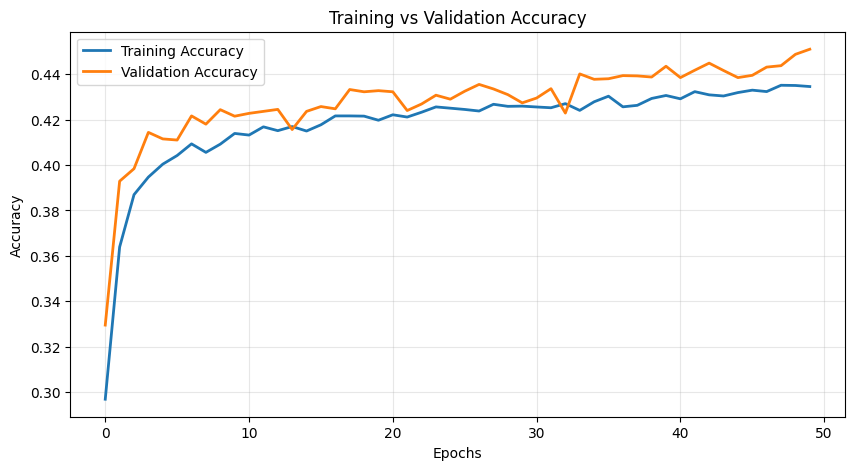
\includegraphics[keepaspectratio]{main_files/figure-pdf/cell-41-output-1.png}}

\subsubsection{Used SHAP to interpret the neural network's
predictions.}\label{used-shap-to-interpret-the-neural-networks-predictions.}

A SHAP explainer was created using a sample of the training data as
background. It computes SHAP values to measure how much each feature
contributes to the model's predictions. Finally, a summary plot is
generated to visualize the global feature importance and understand
which features have the greatest impact on the model's decisions.

\begin{Shaded}
\begin{Highlighting}[]
\NormalTok{X\_sample }\OperatorTok{=}\NormalTok{ X\_test\_scaled[:}\DecValTok{300}\NormalTok{]}
\end{Highlighting}
\end{Shaded}

\begin{Shaded}
\begin{Highlighting}[]
\KeywordTok{def}\NormalTok{ predict\_fn(data):}
    \ControlFlowTok{return}\NormalTok{ model.predict(data, verbose}\OperatorTok{=}\DecValTok{0}\NormalTok{)}

\NormalTok{background }\OperatorTok{=}\NormalTok{ shap.sample(X\_train\_scaled, }\DecValTok{100}\NormalTok{, random\_state}\OperatorTok{=}\DecValTok{42}\NormalTok{)}
\NormalTok{explainer }\OperatorTok{=}\NormalTok{ shap.KernelExplainer(predict\_fn, background)}
\end{Highlighting}
\end{Shaded}

\begin{Shaded}
\begin{Highlighting}[]
\NormalTok{shap\_values }\OperatorTok{=}\NormalTok{ explainer.shap\_values(background[:}\DecValTok{10}\NormalTok{])}
\end{Highlighting}
\end{Shaded}

\begin{verbatim}
  0%|          | 0/10 [00:00<?, ?it/s]
\end{verbatim}

\subsection{🧠 Model Explainability: Global Feature
Importance}\label{model-explainability-global-feature-importance}

\subsubsection{📊 SHAP Summary Plot}\label{shap-summary-plot}

This plot displays the \textbf{global feature importance} for the model,
as calculated by SHAP (SHapley Additive exPlanations). The features on
the y-axis are ranked from the most impactful (top) to the least
impactful (bottom).

The x-axis, labeled
\texttt{mean(\textbar{}SHAP\ value\textbar{})\ (average\ impact\ on\ model\ output\ magnitude)},
quantifies the average absolute effect each feature has on the model's
predictions. A longer bar signifies a feature with a greater overall
influence. The multi-colored segments break down this total impact,
showing the contribution from each specific region (e.g., North America,
Middle East).

\subsubsection{📈 Key Insights:}\label{key-insights}

\begin{itemize}
\tightlist
\item
  \textbf{Most Important Feature:} \texttt{diff\_overall\_vs\_star} is
  decisively the most influential feature the model relies on to make
  its predictions, with an average impact value of approximately 0.60.
\item
  \textbf{Top-Tier Features:} The engineered ``difference'' features
  (\texttt{diff\_facilities}, \texttt{diff\_value\_for\_money},
  \texttt{diff\_cleanliness}, \texttt{diff\_location},
  \texttt{diff\_comfort}) are the next most dominant factors, with
  impact values ranging from \textasciitilde0.26 to \textasciitilde0.32.
\item
  \textbf{Mid-Tier Features:} The \texttt{traveller\_type\_} features
  (Solo, Couple, Family) and \texttt{diff\_staff} hold moderate
  predictive power, with impact values between \textasciitilde0.18 and
  \textasciitilde0.21.
\item
  \textbf{Negligible Features:} \texttt{age},
  \texttt{user\_gender\_Male}, and \texttt{user\_gender\_Other} have
  \textbf{near-zero impact} on the model's output (\textasciitilde0.01
  or less). This suggests they provide minimal predictive value for this
  task.
\item
  \textbf{Regional Impact Distribution:}

  \begin{itemize}
  \tightlist
  \item
    For \texttt{diff\_overall\_vs\_star}, the impact is distributed
    across multiple regions, with substantial contributions from
    \textbf{Middle\_East} (blue), \textbf{Western\_Europe} (light blue),
    \textbf{Africa} (purple), \textbf{South\_America} (pink/magenta),
    and \textbf{Southeast\_Asia} (hot pink).
  \item
    \textbf{Middle\_East} shows consistent, significant contribution
    across all top ``difference'' features, indicating this region's
    data plays a key role in the model's learning.
  \item
    Regional patterns vary across features, suggesting geographic
    differences in what drives hotel satisfaction.
  \end{itemize}
\end{itemize}

\subsubsection{💡 Interpretation:}\label{interpretation}

The dominance of difference features (especially
\texttt{diff\_overall\_vs\_star}) indicates that \textbf{discrepancies
between expected and actual hotel performance} are the primary drivers
of the model's predictions. This suggests the model is likely predicting
satisfaction levels or review scores based on how well hotels meet
expectations relative to their star rating. The minimal impact of
demographic features (age and gender) implies that satisfaction patterns
are more universal across different traveler demographics than they are
influenced by individual characteristics.

\begin{Shaded}
\begin{Highlighting}[]
\NormalTok{country\_names }\OperatorTok{=}\NormalTok{ le.classes\_.tolist()}
\NormalTok{shap.summary\_plot(}
\NormalTok{    shap\_values,}
\NormalTok{    X\_sample[:}\DecValTok{100}\NormalTok{],}
\NormalTok{    feature\_names}\OperatorTok{=}\NormalTok{X.columns,}
\NormalTok{    plot\_type}\OperatorTok{=}\StringTok{"bar"}\NormalTok{,}
\NormalTok{    class\_names}\OperatorTok{=}\NormalTok{country\_names,}
\NormalTok{    show}\OperatorTok{=}\VariableTok{False}
\NormalTok{)}

\NormalTok{plt.title(}\StringTok{"Global Feature Importance (SHAP Summary)"}\NormalTok{, fontsize}\OperatorTok{=}\DecValTok{14}\NormalTok{, fontweight}\OperatorTok{=}\StringTok{\textquotesingle{}bold\textquotesingle{}}\NormalTok{)}
\NormalTok{plt.tight\_layout()}
\NormalTok{plt.show()}
\end{Highlighting}
\end{Shaded}

\begin{verbatim}
C:\Users\abdel\AppData\Local\Temp\ipykernel_4916\3419342718.py:2: FutureWarning: The NumPy global RNG was seeded by calling `np.random.seed`. In a future version this function will no longer use the global RNG. Pass `rng` explicitly to opt-in to the new behaviour and silence this warning.
  shap.summary_plot(
\end{verbatim}

\pandocbounded{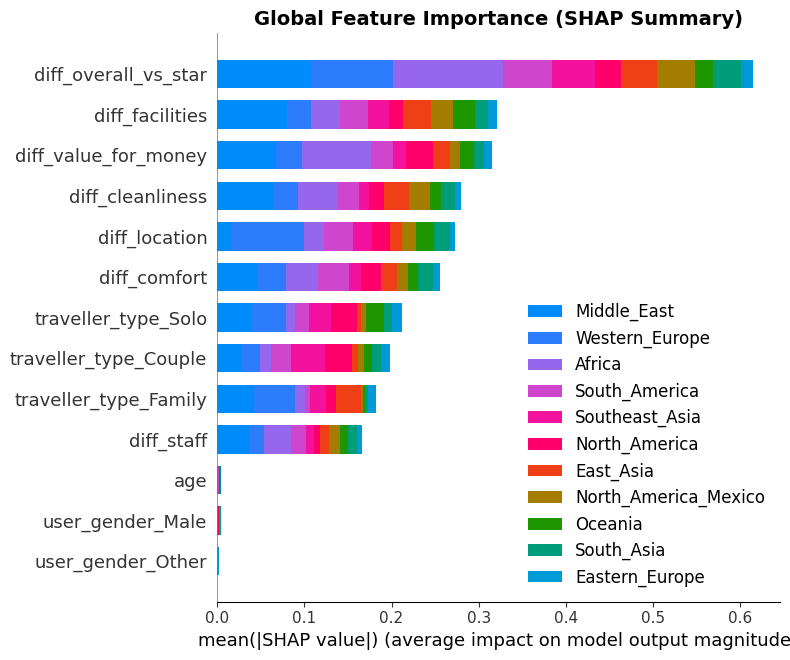
\includegraphics[keepaspectratio]{main_files/figure-pdf/cell-45-output-2.png}}

\subsubsection{Generated a local explanation using
LIME.}\label{generated-a-local-explanation-using-lime.}

LIME provides an interpretable, instance-level explanation by
identifying the most influential features that contributed to a specific
prediction made by the neural network. This helps understand why the
model predicted a certain class for a given input sample.

\subsection{🔬 Model Explainability: Local Prediction
Analysis}\label{model-explainability-local-prediction-analysis}

\subsubsection{📊 Local Explanation Plot (Explaining the ``East Asia''
Prediction)}\label{local-explanation-plot-explaining-the-east-asia-prediction}

This plot explains \emph{why} the model made a specific prediction for a
single data instance (instance 157/157). The central ``waterfall'' chart
shows which features pushed the model's prediction \emph{towards} ``East
Asia'' (light blue) and which pushed it \emph{away} (pink, ``NOT East
Asia'').

The final prediction score for ``East Asia'' is \textbf{0.18}, which is
the result of the ``battle'' between these positive and negative feature
contributions.

\subsubsection{🧾 Final Prediction
Probabilities}\label{final-prediction-probabilities}

For this specific instance, the model's top predictions were:

\begin{itemize}
\tightlist
\item
  \textbf{Western\_Europe: 0.27 (Highest probability)}
\item
  Other: 0.23
\item
  Southeast\_Asia: 0.18
\item
  \textbf{East\_Asia: 0.18 (This is the class being explained)}
\item
  Africa: 0.14
\end{itemize}

\subsubsection{📈 Key Drivers for This Specific
Prediction}\label{key-drivers-for-this-specific-prediction}

\paragraph{\texorpdfstring{👎 Factors Pushing \emph{AWAY} from ``East
Asia'' (Negative
Impact)}{👎 Factors Pushing AWAY from ``East Asia'' (Negative Impact)}}\label{factors-pushing-away-from-east-asia-negative-impact}

These features provided the strongest evidence \emph{against} this
instance being ``East Asia'':

\begin{enumerate}
\def\labelenumi{\arabic{enumi}.}
\tightlist
\item
  \textbf{\texttt{traveller\_type\_Family}}: This was the most
  significant negative factor, with an impact of -0.06. The instance's
  value for this was -0.56.
\item
  \textbf{\texttt{diff\_facilities}}: This had the second-strongest
  negative impact (-0.05). The instance's value was -1.13, which
  triggered the \texttt{diff\_facilities\ \textless{}=\ -0.70} rule.
\item
  \textbf{\texttt{diff\_overall\_vs\_star}}: Had a negative impact of
  -0.03.
\item
  \textbf{\texttt{traveller\_type\_Solo}}: Also had a negative impact of
  -0.03.
\end{enumerate}

\paragraph{\texorpdfstring{👍 Factors Pushing \emph{TOWARDS} ``East
Asia'' (Positive
Impact)}{👍 Factors Pushing TOWARDS ``East Asia'' (Positive Impact)}}\label{factors-pushing-towards-east-asia-positive-impact}

These features provided the strongest evidence \emph{for} this instance
being ``East Asia'':

\begin{enumerate}
\def\labelenumi{\arabic{enumi}.}
\tightlist
\item
  \textbf{\texttt{diff\_cleanliness}}: This was the single most powerful
  \emph{positive} feature, with an impact of +0.03. The instance's value
  was 1.11, triggering the
  \texttt{diff\_cleanliness\ \textgreater{}\ 0.70} rule.
\item
  \textbf{\texttt{traveller\_type\_Couple}}: This had a small positive
  impact (+0.01). The instance's value was 1.38.
\end{enumerate}

\subsubsection{⚖️ Overall Conclusion}\label{overall-conclusion}

For this traveller, the model's prediction for ``East Asia'' was low
(0.18) because the negative factors (especially
\texttt{traveller\_type\_Family} and \texttt{diff\_facilities})
\textbf{strongly outweighed} the positive factors (like
\texttt{diff\_cleanliness}). Even though this traveller had a high
cleanliness score (1.11), which is evidence for ``East Asia'', it was
not enough to overcome the negative evidence from other features.

\begin{Shaded}
\begin{Highlighting}[]
\NormalTok{explainer }\OperatorTok{=}\NormalTok{ lime\_tabular.LimeTabularExplainer(}
\NormalTok{    training\_data}\OperatorTok{=}\NormalTok{np.array(X\_train\_scaled),}
\NormalTok{    feature\_names}\OperatorTok{=}\NormalTok{X.columns,}
\NormalTok{    class\_names}\OperatorTok{=}\NormalTok{le.classes\_,}
\NormalTok{    mode}\OperatorTok{=}\StringTok{\textquotesingle{}classification\textquotesingle{}}
\NormalTok{)}


\NormalTok{i }\OperatorTok{=} \DecValTok{0}
\NormalTok{sample }\OperatorTok{=}\NormalTok{ X\_test\_scaled[i].reshape(}\DecValTok{1}\NormalTok{, }\OperatorTok{{-}}\DecValTok{1}\NormalTok{)}


\NormalTok{exp }\OperatorTok{=}\NormalTok{ explainer.explain\_instance(}
\NormalTok{    data\_row}\OperatorTok{=}\NormalTok{X\_test\_scaled[i],}
\NormalTok{    predict\_fn}\OperatorTok{=}\NormalTok{model.predict,}
\NormalTok{    num\_features}\OperatorTok{=}\DecValTok{13}  
\NormalTok{)}

\NormalTok{exp.show\_in\_notebook(show\_table}\OperatorTok{=}\VariableTok{True}\NormalTok{)}
\end{Highlighting}
\end{Shaded}

\begin{verbatim}
157/157 ━━━━━━━━━━━━━━━━━━━━ 0s 724us/step
\end{verbatim}

\begin{verbatim}
<IPython.core.display.HTML object>
\end{verbatim}

\subsubsection{Implemented an inference function that processes raw user
input, prepares it in the same format used during training, and predicts
the corresponding country group using the trained neural
network.}\label{implemented-an-inference-function-that-processes-raw-user-input-prepares-it-in-the-same-format-used-during-training-and-predicts-the-corresponding-country-group-using-the-trained-neural-network.}

The function handles feature encoding, scaling, and outputs both the
predicted class and the model's confidence scores for each group.

\begin{Shaded}
\begin{Highlighting}[]
\KeywordTok{def}\NormalTok{ predict\_country\_group(}\BuiltInTok{raw\_input}\NormalTok{):}

\NormalTok{    age\_group\_map }\OperatorTok{=}\NormalTok{ \{}
        \StringTok{"18{-}25"}\NormalTok{: }\DecValTok{1}\NormalTok{,}
        \StringTok{"26{-}35"}\NormalTok{: }\DecValTok{2}\NormalTok{,}
        \StringTok{"36{-}45"}\NormalTok{: }\DecValTok{3}\NormalTok{,}
        \StringTok{"46{-}55"}\NormalTok{: }\DecValTok{4}\NormalTok{,}
        \StringTok{"56+"}\NormalTok{: }\DecValTok{5}
\NormalTok{    \}}
\NormalTok{    age\_value }\OperatorTok{=}\NormalTok{ age\_group\_map.get(}\BuiltInTok{raw\_input}\NormalTok{.get(}\StringTok{"age\_group"}\NormalTok{), }\DecValTok{3}\NormalTok{)  }\CommentTok{\# default: 36{-}45}

\NormalTok{    diff\_overall\_vs\_star }\OperatorTok{=} \BuiltInTok{raw\_input}\NormalTok{[}\StringTok{"score\_overall"}\NormalTok{] }\OperatorTok{{-}} \BuiltInTok{raw\_input}\NormalTok{[}\StringTok{"star\_rating"}\NormalTok{]}
\NormalTok{    diff\_cleanliness }\OperatorTok{=} \BuiltInTok{raw\_input}\NormalTok{[}\StringTok{"score\_cleanliness"}\NormalTok{] }\OperatorTok{{-}} \BuiltInTok{raw\_input}\NormalTok{[}\StringTok{"cleanliness\_base"}\NormalTok{]}
\NormalTok{    diff\_comfort }\OperatorTok{=} \BuiltInTok{raw\_input}\NormalTok{[}\StringTok{"score\_comfort"}\NormalTok{] }\OperatorTok{{-}} \BuiltInTok{raw\_input}\NormalTok{[}\StringTok{"comfort\_base"}\NormalTok{]}
\NormalTok{    diff\_facilities }\OperatorTok{=} \BuiltInTok{raw\_input}\NormalTok{[}\StringTok{"score\_facilities"}\NormalTok{] }\OperatorTok{{-}} \BuiltInTok{raw\_input}\NormalTok{[}\StringTok{"facilities\_base"}\NormalTok{]}
\NormalTok{    diff\_location }\OperatorTok{=} \BuiltInTok{raw\_input}\NormalTok{[}\StringTok{"score\_location"}\NormalTok{] }\OperatorTok{{-}} \BuiltInTok{raw\_input}\NormalTok{[}\StringTok{"location\_base"}\NormalTok{]}
\NormalTok{    diff\_staff }\OperatorTok{=} \BuiltInTok{raw\_input}\NormalTok{[}\StringTok{"score\_staff"}\NormalTok{] }\OperatorTok{{-}} \BuiltInTok{raw\_input}\NormalTok{[}\StringTok{"staff\_base"}\NormalTok{]}
\NormalTok{    diff\_value\_for\_money }\OperatorTok{=} \BuiltInTok{raw\_input}\NormalTok{[}\StringTok{"score\_value\_for\_money"}\NormalTok{] }\OperatorTok{{-}} \BuiltInTok{raw\_input}\NormalTok{[}\StringTok{"value\_for\_money\_base"}\NormalTok{]}

\NormalTok{    model\_input }\OperatorTok{=}\NormalTok{ \{}
        \StringTok{"diff\_overall\_vs\_star"}\NormalTok{: diff\_overall\_vs\_star,}
        \StringTok{"diff\_cleanliness"}\NormalTok{: diff\_cleanliness,}
        \StringTok{"diff\_comfort"}\NormalTok{: diff\_comfort,}
        \StringTok{"diff\_facilities"}\NormalTok{: diff\_facilities,}
        \StringTok{"diff\_location"}\NormalTok{: diff\_location,}
        \StringTok{"diff\_staff"}\NormalTok{: diff\_staff,}
        \StringTok{"diff\_value\_for\_money"}\NormalTok{: diff\_value\_for\_money,}
        \StringTok{"traveller\_type\_Couple"}\NormalTok{: }\DecValTok{1} \ControlFlowTok{if} \BuiltInTok{raw\_input}\NormalTok{[}\StringTok{"traveller\_type"}\NormalTok{] }\OperatorTok{==} \StringTok{"Couple"} \ControlFlowTok{else} \DecValTok{0}\NormalTok{,}
        \StringTok{"traveller\_type\_Family"}\NormalTok{: }\DecValTok{1} \ControlFlowTok{if} \BuiltInTok{raw\_input}\NormalTok{[}\StringTok{"traveller\_type"}\NormalTok{] }\OperatorTok{==} \StringTok{"Family"} \ControlFlowTok{else} \DecValTok{0}\NormalTok{,}
        \StringTok{"traveller\_type\_Solo"}\NormalTok{: }\DecValTok{1} \ControlFlowTok{if} \BuiltInTok{raw\_input}\NormalTok{[}\StringTok{"traveller\_type"}\NormalTok{] }\OperatorTok{==} \StringTok{"Solo"} \ControlFlowTok{else} \DecValTok{0}\NormalTok{,}
        \StringTok{"user\_gender\_Male"}\NormalTok{: }\DecValTok{1} \ControlFlowTok{if} \BuiltInTok{raw\_input}\NormalTok{[}\StringTok{"user\_gender"}\NormalTok{] }\OperatorTok{==} \StringTok{"Male"} \ControlFlowTok{else} \DecValTok{0}\NormalTok{,}
        \StringTok{"user\_gender\_Other"}\NormalTok{: }\DecValTok{1} \ControlFlowTok{if} \BuiltInTok{raw\_input}\NormalTok{[}\StringTok{"user\_gender"}\NormalTok{] }\OperatorTok{==} \StringTok{"Other"} \ControlFlowTok{else} \DecValTok{0}\NormalTok{,}
        \StringTok{"age"}\NormalTok{: age\_value}
\NormalTok{    \}}

\NormalTok{    feature\_columns }\OperatorTok{=}\NormalTok{ [}
        \StringTok{\textquotesingle{}diff\_overall\_vs\_star\textquotesingle{}}\NormalTok{, }\StringTok{\textquotesingle{}diff\_cleanliness\textquotesingle{}}\NormalTok{, }\StringTok{\textquotesingle{}diff\_comfort\textquotesingle{}}\NormalTok{,}
        \StringTok{\textquotesingle{}diff\_facilities\textquotesingle{}}\NormalTok{, }\StringTok{\textquotesingle{}diff\_location\textquotesingle{}}\NormalTok{, }\StringTok{\textquotesingle{}diff\_staff\textquotesingle{}}\NormalTok{,}
        \StringTok{\textquotesingle{}diff\_value\_for\_money\textquotesingle{}}\NormalTok{, }\StringTok{\textquotesingle{}traveller\_type\_Couple\textquotesingle{}}\NormalTok{,}
        \StringTok{\textquotesingle{}traveller\_type\_Family\textquotesingle{}}\NormalTok{, }\StringTok{\textquotesingle{}traveller\_type\_Solo\textquotesingle{}}\NormalTok{,}
        \StringTok{\textquotesingle{}user\_gender\_Male\textquotesingle{}}\NormalTok{, }\StringTok{\textquotesingle{}user\_gender\_Other\textquotesingle{}}\NormalTok{, }\StringTok{\textquotesingle{}age\textquotesingle{}}
\NormalTok{    ]}

\NormalTok{    input\_df }\OperatorTok{=}\NormalTok{ pd.DataFrame([model\_input])[feature\_columns]}
\NormalTok{    scaled\_input }\OperatorTok{=}\NormalTok{ scaler.transform(input\_df)}


\NormalTok{    probs }\OperatorTok{=}\NormalTok{ model.predict(scaled\_input)}
\NormalTok{    predicted\_class }\OperatorTok{=}\NormalTok{ np.argmax(probs, axis}\OperatorTok{=}\DecValTok{1}\NormalTok{)[}\DecValTok{0}\NormalTok{]}
\NormalTok{    predicted\_group }\OperatorTok{=}\NormalTok{ le.inverse\_transform([predicted\_class])[}\DecValTok{0}\NormalTok{]}

    \BuiltInTok{print}\NormalTok{(}\SpecialStringTok{f"}\CharTok{\textbackslash{}n}\SpecialStringTok{Predicted Country Group: }\SpecialCharTok{\{}\NormalTok{predicted\_group}\SpecialCharTok{\}}\CharTok{\textbackslash{}n}\SpecialStringTok{"}\NormalTok{)}
    \BuiltInTok{print}\NormalTok{(}\StringTok{"Class Probabilities:"}\NormalTok{)}
    \ControlFlowTok{for}\NormalTok{ cls, prob }\KeywordTok{in} \BuiltInTok{zip}\NormalTok{(le.classes\_, probs[}\DecValTok{0}\NormalTok{]):}
        \BuiltInTok{print}\NormalTok{(}\SpecialStringTok{f"  }\SpecialCharTok{\{}\NormalTok{cls}\SpecialCharTok{\}}\SpecialStringTok{: }\SpecialCharTok{\{}\BuiltInTok{float}\NormalTok{(prob)}\SpecialCharTok{:.3f\}}\SpecialStringTok{"}\NormalTok{)}

    \ControlFlowTok{return}\NormalTok{ \{}
        \StringTok{"predicted\_group"}\NormalTok{: predicted\_group,}
        \StringTok{"probabilities"}\NormalTok{: \{cls: }\BuiltInTok{float}\NormalTok{(prob) }\ControlFlowTok{for}\NormalTok{ cls, prob }\KeywordTok{in} \BuiltInTok{zip}\NormalTok{(le.classes\_, probs[}\DecValTok{0}\NormalTok{])\}}
\NormalTok{    \}}
\end{Highlighting}
\end{Shaded}

\begin{Shaded}
\begin{Highlighting}[]
\NormalTok{sample\_input }\OperatorTok{=}\NormalTok{ \{}
    \StringTok{"age\_group"}\NormalTok{: }\StringTok{"26{-}35"}\NormalTok{,}
    \StringTok{"user\_gender"}\NormalTok{: }\StringTok{"Female"}\NormalTok{,}
    \StringTok{"traveller\_type"}\NormalTok{: }\StringTok{"Solo"}\NormalTok{,}
    \StringTok{"score\_overall"}\NormalTok{: }\FloatTok{8.7}\NormalTok{,}
    \StringTok{"star\_rating"}\NormalTok{: }\DecValTok{5}\NormalTok{,}
    \StringTok{"score\_cleanliness"}\NormalTok{: }\FloatTok{8.5}\NormalTok{,}
    \StringTok{"cleanliness\_base"}\NormalTok{: }\FloatTok{9.0}\NormalTok{,}
    \StringTok{"score\_comfort"}\NormalTok{: }\FloatTok{8.2}\NormalTok{,}
    \StringTok{"comfort\_base"}\NormalTok{: }\FloatTok{8.5}\NormalTok{,}
    \StringTok{"score\_facilities"}\NormalTok{: }\FloatTok{7.8}\NormalTok{,}
    \StringTok{"facilities\_base"}\NormalTok{: }\FloatTok{8.0}\NormalTok{,}
    \StringTok{"score\_location"}\NormalTok{: }\FloatTok{8.9}\NormalTok{,}
    \StringTok{"location\_base"}\NormalTok{: }\FloatTok{9.3}\NormalTok{,}
    \StringTok{"score\_staff"}\NormalTok{: }\FloatTok{9.1}\NormalTok{,}
    \StringTok{"staff\_base"}\NormalTok{: }\FloatTok{9.0}\NormalTok{,}
    \StringTok{"score\_value\_for\_money"}\NormalTok{: }\FloatTok{8.4}\NormalTok{,}
    \StringTok{"value\_for\_money\_base"}\NormalTok{: }\FloatTok{8.0}
\NormalTok{\}}

\NormalTok{result }\OperatorTok{=}\NormalTok{ predict\_country\_group(sample\_input)}
\end{Highlighting}
\end{Shaded}

\begin{verbatim}
1/1 ━━━━━━━━━━━━━━━━━━━━ 0s 28ms/step

Predicted Country Group: North_America

Class Probabilities:
  Africa: 0.001
  East_Asia: 0.000
  Eastern_Europe: 0.000
  Middle_East: 0.000
  North_America: 0.339
  North_America_Mexico: 0.002
  Oceania: 0.002
  South_America: 0.253
  South_Asia: 0.321
  Southeast_Asia: 0.000
  Western_Europe: 0.082
\end{verbatim}

\begin{Shaded}
\begin{Highlighting}[]
\NormalTok{sample\_input }\OperatorTok{=}\NormalTok{ \{}
    \StringTok{"age\_group"}\NormalTok{: }\StringTok{"36{-}45"}\NormalTok{,}
    \StringTok{"user\_gender"}\NormalTok{: }\StringTok{"Male"}\NormalTok{,}
    \StringTok{"traveller\_type"}\NormalTok{: }\StringTok{"Solo"}\NormalTok{,}

    \CommentTok{\# Raw scores vs base values (chosen to produce the same diffs)}
    \StringTok{"score\_overall"}\NormalTok{: }\FloatTok{8.8}\NormalTok{,}
    \StringTok{"star\_rating"}\NormalTok{: }\FloatTok{5.0}\NormalTok{,                      }\CommentTok{\# 8.8 {-} 5.0 = 3.8}

    \StringTok{"score\_cleanliness"}\NormalTok{: }\FloatTok{8.0}\NormalTok{,}
    \StringTok{"cleanliness\_base"}\NormalTok{: }\FloatTok{8.5}\NormalTok{,                 }\CommentTok{\# diff = {-}0.5}

    \StringTok{"score\_comfort"}\NormalTok{: }\FloatTok{7.6}\NormalTok{,}
    \StringTok{"comfort\_base"}\NormalTok{: }\FloatTok{8.0}\NormalTok{,                     }\CommentTok{\# diff = {-}0.4}

    \StringTok{"score\_facilities"}\NormalTok{: }\FloatTok{7.4}\NormalTok{,}
    \StringTok{"facilities\_base"}\NormalTok{: }\FloatTok{8.0}\NormalTok{,                  }\CommentTok{\# diff = {-}0.6}

    \StringTok{"score\_location"}\NormalTok{: }\FloatTok{8.9}\NormalTok{,}
    \StringTok{"location\_base"}\NormalTok{: }\FloatTok{9.0}\NormalTok{,                    }\CommentTok{\# diff = {-}0.1}

    \StringTok{"score\_staff"}\NormalTok{: }\FloatTok{9.7}\NormalTok{,}
    \StringTok{"staff\_base"}\NormalTok{: }\FloatTok{9.0}\NormalTok{,                       }\CommentTok{\# diff = +0.7}

    \StringTok{"score\_value\_for\_money"}\NormalTok{: }\FloatTok{8.3}\NormalTok{,}
    \StringTok{"value\_for\_money\_base"}\NormalTok{: }\FloatTok{8.0}              \CommentTok{\# diff = +0.3}
\NormalTok{\}}


\NormalTok{result }\OperatorTok{=}\NormalTok{ predict\_country\_group(sample\_input)}
\end{Highlighting}
\end{Shaded}

\begin{verbatim}
1/1 ━━━━━━━━━━━━━━━━━━━━ 0s 28ms/step

Predicted Country Group: South_America

Class Probabilities:
  Africa: 0.000
  East_Asia: 0.000
  Eastern_Europe: 0.000
  Middle_East: 0.017
  North_America: 0.107
  North_America_Mexico: 0.001
  Oceania: 0.042
  South_America: 0.365
  South_Asia: 0.278
  Southeast_Asia: 0.000
  Western_Europe: 0.189
\end{verbatim}




\end{document}
